%======================================================================
%   Zak Webb
%   Ph.D. Thesis
%   Department of Physics and Astronomy
%   University of Waterloo
% 
%   Universality of multi-particle scattering
%======================================================================


\documentclass[../thesis-main/thesis-main]{subfiles}
\begin{document}
 
\chapter{Multi-particle quantum walk}
\label{chap:MPQW}

So far, we have only focused on the case of a single walker moving on a graph.  These systems exhibit all the hallmarks of quantum systems, with superpositions of states, entanglement, and the like, but neccessity forces the corresponding graphs to be unphysical; as each vertex corresponds to a computational basis state, in order to get nontrivial computational power we are forced to work on graphs that are not practical to implement in the real world.

From a computational point of view, this does not matter.  \chap{SP_universality} showed that quantum walk is universal for quantum computation, and thus we wouldn't expect it to be easier to implement than a universal quantum computer.  However, several experimental implementations of quantum walk have been carried out \cite{DSBEFFMZ05, KFC09, PLP08}, where the encoding has been done in a non-scalable manner.  

Continuing in this manner, experimentalists have also examined what happens when multiple particles interact on the same graph.  Explicitly, they have analyzed what happens when two bosons walk on a graph \cite{BLMS09, PLM10,SSVMCRO12}, what happens when multiple bosons move along a long path, and various other simple experiments.

While these experimental realizations of multi-particle quantum walk have flourished, the theoretical side has only seen some small development.  In particular, there have been attempts to use these MPQW as tools for analyzing graph properties, in the hope that they might be useful for the graph isomorphism problem, but many of these avenues have been proven impossible.  Additionally, there are some continuous space analysis on the eigenstates of some interaction Hamiltonians, but in most cases no closed form solution exists.

In this chapter, we will define our model of multi-particle quantum walk, and analyze the dynamics of such a model on some simple systems.  While this will not improve drastically our previous knowledge this does give us a better understanding of simple interactions.

Note that this chapter takes results from Childs, Gosset, and Webb \cite{MPQW,BHQMA}, and improves some of the results from those papers as well.  We will mention explicitly where the results in this thesis improve previous results.


\section{Multi-particle quantum walk}

In \chap{scattering_on_graphs}, we analyzed a single-particle quantum walk, and in particular we found that the evolution proceeds with a Hamiltonian given by the adjacency matrix of the graph.  If we want to generalize this framework to multiple particles, we will want to ensure that each individual particle in our framework evolves as in the single-particle case.

Namely, we had that the Hilbert space for the single-particle quantum walk on a graph $G$ was given by $\CC^{|V(G)|}$, with the computational basis given by the states labeled by the vertices of the graph:
\begin{align}
  \big\{ \ket{v}: v\in V(G)\big\}.
\end{align}
If we want to extend this to multiple particles, we shall take multiple copies of this Hilbert space.  As such, we will assume that Hilbert space for the $N$-particle quantum walk on a graph $G$ is $\CC^{|V(G)|^N}$, with the computational basis given by
\begin{align}
  \big\{ \ket{v_1,v_2,\cdots,v_N} : \forall i \in [N], v_i\in V(G)\big\}.
\end{align}
Note that for the moment we assume that the $N$ particles are distinguishable.

Now that we have a Hilbert space for the $N$-particle quantum walk, we still need the Hamiltonian to understand the time-evolution.  As the Hamiltonian for a single particle is simply the adjacency matrix of the graph $G$, we will take as our definition of the $N$-particle quantum walk (without interaction) as a sum of Hamiltonians that each generate the correct single-particle evolution for a given particle.  Namely, we have that the $N$ particle quantum walk with no interaction takes the form
\begin{align}
  H_{\text{mov}}^N = \sum_{w\in [N]} A(G)^{(w)} \label{eq:MPQW_movement}
\end{align}
where for a given single-particle operator $B$, we represent by $B^{(w)}$ the operator that acts on $N$ particles as $B$ on the $w$th particle and $\II$ on the rest.  With such a Hamiltonian, the evolution operator decomposes into a product of commuting terms, where each term acts as the single particle evolution for a different particle, exactly as we want.

While this definition of an $N$-particle quantum walk does nicely generalize that of a single-particle quantum walk, it is not any more interesting than the original single-particle walk.  In particular, the eigenstates of \eq{MPQW_movement} easily decompose into product states, where each of the individual particles are in an eigenstate of $A(G)$.  Such a system is only as computationally powerful as that of a single-particle system, since we can simulate the $N$-particle system via $N$ single-particle evolutions.  To get around this, we will thus want to force some interaction between the particles. We will also want to ensure that we capture the intuitive structure of particle interactions from the continuum, so that our model makes sense as a quantum walk.  Note that in the continuum, the interaction strength only depends on the distance between the particles.  This translation invariance can have several different abstractions to a general graph (which could be thought of as something related to the Bohm-Aharanov effect), but on a one dimensional lattice we would expect the interaction to only depend on the distance between the particles, as measured by the shortest path between vertices.

We will take this requirement on the infinite path and use it for all vertices.  Further, we will assume some finite range of interaction, so that particles with large physical separation don't interact.   Namely, let us choose some $\dmax \in \NN$ to be the finite range of the interaction, and then choose $d+1$ symmetric polynomials in two variables, $U_{d}$, for $0\leq d \leq \dmax$.  Additionally, assuming that we know that there are a total of $N$ particles, let $\hat{n}_v$ for $v\in V(G)$ be the operator that counts the number of particles at vertex $v$, explicitly given by 
\begin{align}
  \hat{n}_v = \sum_{w\in [N]} \ketbra{v}{v}^{(w)}.\label{eq:n_hat}
\end{align}
With these values, and if $d(u,v)$ is the distance function on the graph $G$ given by the length of the shortest path between $u$ and $v$, we can define the interaction
\begin{align}
  H_{\text{int}} = \sum_{d=0}^{\dmax} \sum_{\substack{ u,v\in V(G)\\d(u,v) = d}}U_{d} (\hat{n}_u,\hat{n}_v).\label{eq:MPQW_int}
\end{align}
Note that on the infinite path (and in fact on any lattice), this interaction has the form we require.

With such a chosen interaction, (i.e., with $\dmax$ and the $U_d$ well defined), we can then define the $N$-particle quantum walk on $G$ with this interaction.  Namely, we let 
\begin{align}
  H_G^N = H_{\text{mov}}^N + H_{\text{int}}^N = \sum_{w\in [N]} A(G)^{(w)} + \sum_{d=0}^{\dmax}  \sum_{\substack{ u,v\in V(G)\\d(u,v) = d}}U_{d} (\hat{n}_u,\hat{n}_v). 
  \label{eq:MPQW_H_defn}
\end{align}
Hamiltonians of this form will be the study of this thesis.  Note that we call the component of \eq{MPQW_H_defn} corresponding to the sum of adjacency matrices \eq{MPQW_movement} the movement term of the Hamiltonian, while the part corresponding to the interaction \eq{MPQW_int} is called the interaction term.

Several times in the thesis, we will need to reference particular values that the interaction Hamiltonian takes.  As such, we will use as shorthand 
\begin{align}
  \mathcal{U}_{d}^{a,b} = \mathcal{U}_{d} (a,b).
\end{align}

%%%%
\subsection{Indistinguishable particles}

Note that in our definition of MPQW, we assume that the particles are all distinguishable, and thus we can locate each of the $N$ particles.  In many cases of interest, though, we will actually not have this ability, as the particles will be indistinguishable.  One might then think that we would need to change our definition in order to characterize these indistinguishable walks.

This turns out to not be the case, however, as Hamiltonian \eq{MPQW_H_defn} is permutation invariant.  In other words, we have that for any permutation of the underlying particle particles (given by $V_\pi$ for a given permutation $\pi \in S_N$),
\begin{align}
  V_\pi H_{G}^N V_\pi^\dag = H_G^N.
\end{align}
Using this, we can then see that the Hamiltonian preserves the symmetric and anti-symmetric subspaces, corresponding to either fermions or bosons.

As such, if we want to restrict our attention to bosonic multi-particle quantum walk, we simply have that the relevant Hilbert space is
\begin{align}
  \span\Big\{\Sym\big(\ket{v_1,v_2,\cdots,v_N} \big): \forall i\in [N], v_i\in V(G) \Big\},
\end{align}
where
\begin{align}
  \Sym\big(\ket{\phi}\big) = \frac{1}{N!} \sum_{\pi\in S_n} V_\pi \ket{\phi},
\end{align}
but where the Hamiltonian for the walk is still given by \eq{MPQW_H_defn}.  Similarly, we have that fermionic MPQW, the Hilbert space is given by 
\begin{align}
  \span\Big\{\ASym\big(\ket{v_1,v_2,\cdots,v_N} \big): \forall i\in [N], v_i\in V(G) \Big\},
\end{align}
where
\begin{align}
  \Sym\big(\ket{\phi}\big) = \frac{1}{N!} \sum_{\pi\in S_n} \sign(\pi) V_\pi \ket{\phi},
\end{align}
and we again use the same Hamiltonian.

\subsection{Examples}

While \eq{MPQW_H_defn} is a well defined mathematical object for a given graph $G$, interaction range $\dmax$, symmetric polynomials $\mathcal{U}_d$, and a number of particles, $N$, as of yet we haven't given any well-known models that fall into this class of interactions.  However, the idea of translation invariant interactions, in which the interaction does not depend on the particular location of a given particle, is abundant in physics, and thus there are several well-know models that relate to our MPQW.

\subsubsection{Bose-Hubbard model}

The Bose-Hubbard model on a graph, where the particles are taken to be bosons, and there is a given onsite interaction between the particles is probably the first interaction that falls into our class of interactions.  In particular, we have that in the second quantized basis, the Hamiltonian for the Bose-Hubbard model on a graph $G$ is usually given by 
\begin{align}
  H_{G}^{\text{BH}} = t_{\text{hop}} \sum_{i,j\in V(G)} A(G)_{ij} a_i^\dag a_j + J_\text{int} \sum_{k\in V(G)} n_k (n_k - 1), \label{eq:BH_H_Fock}
\end{align}
where $a_i^\dag$ creates a boson at vertex $i$, and $n_i = a_ia_i^\dag$ counts the number of particles at vertex $i$.  Note that this form of the Hamiltonian does not require knowledge of the number of particles, as it works in the Fock space which allows for an arbitrary number of particles.  Additionally, we have that \eq{BH_H_Fock} preserves the number of particles, and thus decomposes into blocks for each particle number.

While this form of \eq{BH_H_Fock} is not quite that of \eq{MPQW_H_defn}, if we assume that there are $N$ particles, we can rewrite the Hamiltonian in the first quantized basis (after restricting to the symmetric subspace) as
\begin{align}
  H_G^{\text{BH},N} = t_{\text{hop}} \sum_{w\in [N]} \sum_{i,j\in V(G)} A_{i,j} \big( \ketbra{i}{j} \big)^{(w)} + J_{\text{int}}\sum_{v\in V(G)}\hat{n}_v\big( \hat{n}_v - 1\big).
\end{align}
This is simply a rescaling by $t_{\text{hop}}$ of a Hamiltonian the form \eq{MPQW_H_defn}, where $\dmax = 0$ and 
\begin{align}
  \mathcal{U}_0(x,y) = \frac{J_{\text{int}}}{4t_{\text{hop}}} (x+y) (x+y-2)
\end{align}

\subsubsection{Nearest-neighbor interactions}

While the Bose-Hubbard model (and onsite-interactions in general) is a well studied model, no onsite-interaction affects the anti-symmetric states at all.  As such, if we want an interaction that will change the structure of the entire Hilbert space, we will need to increase our $\dmax$ to at least 1, arriving at nearest neighbor interactions.  

While there are many different interactions with $\dmax = 1$, probably the most simple is given by $\mathcal{U}_0 = 0$ and 
\begin{align}
  \mathcal{U}_1(x,y) = \gamma xy.
\end{align}
With this interaction, we then have that the corresponding MPQW Hamiltonian is given by
\begin{align}
  H_{G}^{\text{NN},N} = \sum_{w\in [N]} A(G)^{(w)} +  \gamma \sum_{\substack{ \{u,v\}\in E(G)}}\hat{n}_u\hat{n}_v
\end{align}

%
%\subsubsection{XY Hamiltonian}
%
%
%As a particular example, if $\dmax = 0$, and 
%\begin{align}
%  U_0(x,y) = \frac{\gamma }{4}(x + y) (x + y -2) \label{eq:bh_int}
%\end{align}
%we have an onsite interaction with strength $\gamma$, for which, if we restrict our attention to symmetric states, is the Bose-Hubbard Hamiltonian with strength $\frac{\gamma}{2}$.  Similarly, if $\dmax = 1$, $U_0 (x,y) = 0$, and $U_1(x,y) = \gamma xy$, we have a nearest-neighbor interaction with strength $\gamma$.


\subsection{Evolution on disconnected graphs}

While a general result about the eigenstates of an $N$-particle quantum walk on a given graph $G$ might be difficult, we can reason about some properties of the eigenstates and time-evolved states without needing to explicitly calculate the overall form of the eigenstates.  In particular, if a given graph on which the particles walk has some property, then so too might the time-evolved states.

Perhaps the most obvious such property is the connectivity of the graph itself.  In particular, our MPQW Hamiltonian \eq{MPQW_H_defn} only allows particles to move between vertices that have a path between them; if two vertices are not connected in $G$, then the corresponding off-diagonal element of the time evolution unitary will always be zero.

We can use this to decompose the time-evolution unitary into a product of commuting unitaries, each corresponding to a specific component of $G$.  If each of the $N$ particles in a state $\ket{\phi}$ have support only on one component of the graph $G$, then the evolution operator is simply a product of $n_c$-particle MPQW evolutions for each component $G_c$ of $G$, where $n_c$ particles are on the $c$-th component.  Explicitly, we have the following lemma:

\begin{lemma}
  Let $G$ be a disconnected graph with $M$ components, and let us examine the $N$-particle MPQW on $G$.  If $\ket{\psi}$ is an $N$-particle state such that each particle $j$ only has support on the $G_{c_j}$th component of $G$, then 
  \begin{align}
    e^{-i H_G^N t} \ket{\phi} = \prod_{c=1}^M W_{c}^\dag \Big(e^{- i H_{G_c}^{n_c} t } \Big)^{(1,2,\cdots,n_c)} W_{c} \ket{\phi}\label{eq:MPQW_disconnect_evolution}
  \end{align}
  where $n_c$ is the number of particles with support on $G_c$, and $W_c$ is a permutation operator that takes the particles with support on $G_c$ to the first $n_c$ particles.  In the special case where $n_c \leq 1$ for all $c$, this then reduces to
  \begin{align}
    e^{-i H_G^N t} \ket{\phi} = \prod_{j=1}^n \Big( e^{-i A(G_{k_j}) t}\Big)^{(j)} \ket{\phi}.
  \end{align}
\label{lem:disconnected_MPQW}
\end{lemma}
\begin{proof}
  Let us assume an arbitrary ordering on the components of $G$, and let $\ket{\phi} = \ket{v_1,v_2,\cdots , v_N}$ be any $N$-particle basis state on $G$, with $n_c$ particles on the $c$-th component of $G$, and where that the first $n_1$ vertices are in $G_1$, then next $n_2$ vertices are in $G_2$, and continuing for all components of $G$.  Note that for all times $t\in \RR$, $e^{-i A(G) t} \ket{v_i}$ only has support on the component of $G$ to which $v_i$ belongs, and thus $e^{-i A(G) t} \ket{v_i} = e^{-i A(G_{c_j})t} \ket{v_i}$ (with the natural identification between basis vectors in the smaller Hilbert space).

As the interaction term of \eq{MPQW_H_defn} is diagonal in the computational basis, we have that for all times $t$, $e^{-i H_G^N t} \ket{\phi}$ only has support on states 
  \begin{align}
    \big\{ \ket{w_1,\cdots, w_N} : \forall i\in [N],  w_i \in V(G_{c_i}) \big\}.
  \end{align}
  Further, as the interaction in \eq{MPQW_H_defn} is finite range (and vertices in different components have infinite distance), this implies that only particles on the same component can interact, and the interaction is restricted to $H(G_c,n_c)$ for each component.

  
  Combining these two results, we then have that, when restricted to states of the form $\ket{\phi}$, we have that the evolution according to $H_G^N$ is equal to that of
  \begin{align}
    e^{-i H_G^N t} \ket{\phi} = \prod_{c=1}^M \Big(e^{-i H_{G_c}^{n_c} t}\Big)^{(  m_c+1,m_c+2,\cdots, m_c+n_c)} \ket{\phi}, 
  \end{align}
  where $m_c = \sum_{j=1}^{c-1} n_c$. If we then use the fact that $H_G^N$ commutes with all permutations of the underlying particles, and that states of the form $\ket{\phi}$ (and their permutations) span the relevant space, we then have \eq{MPQW_disconnect_evolution}.  If we restrict ourselves to the case where each particle is on a separate component, the second equation follows immediately.
\end{proof}

Note that if we combine this lemma with the truncation lemma (\lem{truncation}), we have that when particles are separated from each other they almost evolve independently, as one might expect.  We will use this intuition several times in the remainder of the thesis.


%%%%%%%%%%%%%%%%%%%%%%%%%%%%%%%
\section{Two-particle scattering on an infinite path}\label{sec:two_particle_scattering}

After choosing a given interaction, equation \eq{MPQW_H_defn} provides us with a well defined MPQW Hamiltonian for $N$-particles.  With this, we can explicitly evolve a given state, and hopefully use such systems for algorithmic advantages.  However, this requires an understanding of the eigenstates of a multi-particle interacting system, for which we have few examples of analytic solutions.  On the other hand, we \emph{can} analyze some highly symmetric systems, when we restrict ourselves to a small number of particles.  Our understanding of these small systems can then be leveraged to gain some information about MPQW with many particles on some given graphs.

In particular, we already know from \chap{scattering_on_graphs} the basic properties of a single particle moving on a long path.  One might expect that that next step would be to understand two particles interacting on a similar scattering graph, but unfortunately even this is a little too complicated for this thesis.  However, we can analyze two particles interacting on an infinite path.

Namely, let us assume that the interaction Hamiltonian has been chosen, such that there is a $\dmax$ and a set of $d+1$ symmetric functions $U_d$.  We can then write the Hamiltonian \eq{MPQW_H_defn} in the basis $\ket{x,y}$, where $x,y\in \ZZ$ are the positions of the first and second particles, as
\begin{align}
  H^{2} = H^1 \otimes \II_y + \II_x \otimes H^1 + \sum_{x\in \ZZ} \sum_{d=0}^{\dmax} U_{d} (\hat{n}_x,\hat{n}_{x+d}) ,
  \label{eq:two_part_H_xy}
\end{align}
where the single-particle Hamiltonian $H^1$ is simply the adjacency matrix for the infinite path, namely
\begin{align}
  H^{1} = \sum_{x\in\ZZ} \ket{x+1}\bra{x} + \ket{x}\bra{x+1}.
\end{align}

Without the interaction term, the eigenstates for this Hamiltonian would simply by two independent scattering eigenstates, with amplitudes of the form $e^{i k_1 x + i k_2y}$.  However, the interaction causes there to be correlations between the two particles, and these correlations will be similar to the single particle interactions scattering off of a graph with two attached semi-infinite paths.  

%As we will eventually be interested in the dynamics of two particles initially prepared in spatially separated wave-packets moving toward each other along the path with momenta $k_1\in(-\pi,0) $ and $k_2\in (0,\pi)$, we will need to understand these scattering eigenstates.  Moreover, as in the single-particle scattering case, the intuition gained from the dynamics will help us in understanding the two-particle scattering eigenstates.

While our given Hamiltonian \eq{two_part_H_xy} is simple to define, in order to understand dynamics we will want to diagonalize it.  Further, while the current basis does have a permutation invariance between the two particles, it does not make use of the translation invariance of the interaction.  To make use of this symmetry, we will need to change to a different basis.

In particular, let us look at the new basis $\ket{s;r}$, where $s = x+y$ and $r = x-y$, and where the allowed values of $(s,r)$ range over those values where $s$ and $r$ are either both even or both odd (i.e., $s+r$ must be even).  If we then expand \eq{two_part_H_xy} in this basis, we find 
\begin{equation}
  H^{(1)}\otimes H^{(1)} + \II\otimes \sum_{r\in \ZZ} \mathcal{V}(|r|) \, \ket{r}\bra{r},
\label{eq:two_part_H_rs}
\end{equation}
where $V(0) = U_0(2,2)$ and $V(r) = U_r(1,1)$ for $r >0$.  

Note that \eq{two_part_H_rs} looks to be much nicer to analyze than \eq{two_part_H_xy}, as we nearly have a separable decomposition of the Hamiltonian.  We do have a decomposition such that the eigenstates corresponding to $s$ don't rely on the current state of $r$, and we will see that once we chose a particular eigenstate for the $s$, the corresponding eigenvalue equation for $r$ will look exactly as a scaled single-particle scattering equation as in \chap{scattering_on_graphs}.

\subsection{Eigenstates on the path}

With the decomposition of \eq{two_part_H_xy} that nicely decouples the center of mass movement from the relative movement of two particles (i.e., the physical meaning of $r$ and $s$), we can determine the eigenvalues and eigenvectors of the Hamiltonian.  

Namely, let us make the ansatz that the eigenstates of \eq{two_part_H_rs} take the form
\begin{align}
  \braket{s;r}{\psi} = e^{ - i p_1 s/2} \braket{r}{\phi_{p_1}}
\end{align}
where $p_1 \in (-\pi,\pi)$.  With this assumption, we then have that the effective Hamiltonian for $\ket{\phi_{p_1}}$ takes the form
\begin{equation}
 2\cos\left(\frac{p_1}{2}\right) H^{(1)}_r + \sum_{r\in \ZZ} \mathcal{V}(|r|) \, \ket{r}\bra{r}.\label{eq:vr_eqn}
\end{equation}
Note that this is simply a rescaled single-particle scattering problem, as in \chap{scattering_on_graphs}, except where the weights of the graph gadget need not be normalized, and with a slight relabeling of the semi-infinite paths (i.e., the paths do not start from $1$).   We can then use the intuition from the chapter to see that for each $p_2\in (0,\pi)$ there is a scattering eigenstate of the form
\begin{equation}
\langle r|\psi (p_1;p_2)\rangle= \begin{cases}  e^{-i p_2 r} + R(p_1,p_2) e^{i p_2 r} &  \text{if } r \leq -\dmax\\
  	f(p_1,p_2,r) &  \text{if } |r| < \dmax\\
  	T(p_1,p_2) e^{- i p_2 r}  & \text{if } r \geq \dmax.\end{cases}
\label{eq:psip1p2}
\end{equation}
for $p_2\in (0,\pi)$. Here the reflection and transmission coefficients $R$ and $T$ and the amplitudes of the scattering state for $|r|<\dmax$ (described by the function $f$) depend on both momenta as well as the interaction $\mathcal{V}$.  With $R$, $T$, and $f$ chosen appropriately, the state $|\mathrm{sc}(p_1;p_2)\rangle$ is an eigenstate of $H^{(2)}$ with eigenvalue $4\cos(p_1/2)\cos(p_2)$.  While it is not possible to give an explicit closed-form solution for all interactions, the form of \eq{psip1p2} will be sufficient for most of our purposes.

Additionally, we can use the fact that $\mathcal{V}(|r|)$ is an even function of $r$ to also define scattering states for $p_2\in (-\pi,0)$ by
\begin{align}
  \langle s;r|\mathrm{sc}(p_1;p_2)\rangle=\langle s;-r|\mathrm{sc}(p_1;-p_2)\rangle.
\end{align}
These other states are obtained by swapping $x$ and $y$, corresponding to interchanging the two particles.

While we will not need a complete basis for for this Hamiltonian, note that if there are any bound states of \eq{vr_eqn}, then there will be corresponding traveling states where the two particles move together.  These are the well known dimer states, and while they are important to find a basis for the entire Hilbert space they will play a role similar to the bound states of single-particle scattering; only exponentially small amplitude of the states of interest will be on these states, and thus we will neglect their study.



The construction of the symmetric and anti-symmetric scattering states follows as one would expect. For $p_1\in (-\pi,\pi)$ and $p_2\in (0,\pi)$, we define
\begin{align}
  \ket{\mathrm{sc}(p_1;p_2)}_\pm = \frac{1}{\sqrt2}\big(\ket{\mathrm{sc}(p_1;p_2)} \pm \ket{\mathrm{sc}(p_1;-p_2)}\big).
\end{align}
If we note that the unitarity of the underlying scattering matrix $S$ and the fact that $V(|r|)$ being even in $r$ forces $R(p_1,p_2) = R(p_1,-p_2)$ and $T(p_1,p_2)  = T(p_1,-p_2)$ we can then see that the combinations
\begin{align}
  |T(p_1,p_2) \pm R(p_1,p_2)| = 1.  
\end{align}
With this, we can then see that the symmeterized scattering states can be expanded as

\begin{align}
    \braket{s;r}{\mathrm{sc}(p_1;p_2)}_\pm
      &= \frac{1}{\sqrt{2}}e^{-i p_1 s/2} \begin{cases}  e^{-i p_2 r} \pm e^{i\theta_{\pm}(p_1,p_2)} e^{i p_2 r} &  \text{if }r \leq- C\\
  	f(p_1,p_2,r) \pm f(p_1,-p_2,-r) & \text{if }  |r| < C\\
	  e^{i\theta_{\pm}(p_1,p_2)} e^{-i p_2 r}\pm e^{i p_2 r}  &  \text{if }r \geq C, \end{cases}
\label{eq:symscatter}
\end{align}
where $\theta_{\pm}(p_1;p_2)$ is a real function defined through
\begin{equation}
e^{i\theta_{\pm}(p_1;p_2)}= T(p_1;p_2)\pm R(p_1;p_2). \label{eq:delta_pm}
\end{equation}


These eigenstates allow us to understand what happens when two particles with momenta $k_1\in(-\pi,0)$ and $k_2\in(0,\pi)$ move toward each other. Here $p_1=-k_1-k_2$ and $p_2=(k_2-k_1)/2$.  Similar to the scattering states of \chap{scattering_on_graphs}, we have that for $|r|\geq C$ the scattering state is a sum of two terms, one corresponding to the two particles moving toward each other and one corresponding to the two particles moving apart after scattering, but where the outgoing term has a  phase of $T\pm R$ relative to the incoming term (as depicted in \fig{wte}). This phase arises from the interaction between the two particles.

In particular, we can transform \eq{symscatter} to the $(x,y)$ basis as
\begin{align}
  &\braket{x,y}{\mathrm{sc}(k_1,k_2)}_{\pm} \nonumber\\
  &\qquad= \frac{1}{\sqrt{2}} e^{i (k_1 + k_2) \frac{x+y}{2}} \begin{cases}  e^{i (k_1 - k_1) \frac{x-y}{2}} \pm e^{i\theta_{\pm}(k_1,k_2)} e^{i (k_2- k_2) \frac{x-y}{2}} &  \text{if }x-y \leq- C\\
  	f\Big(-k_1-k_2,\frac{k_2-k_1}{2},x-y\Big) \pm f(-k_1-k_2,\frac{k_1-k_2}{2},y-x) & \text{if }  |x-y| < C\\
	  e^{i\theta_{\pm}(k_1,k_2)} e^{i (k_1 - k_2) \frac{x-y}{2}}\pm e^{i (k_2- k_1) \frac{x-y}{2}}  &  \text{if }x-y \geq C, \end{cases}
\end{align}
where we defined $\theta_{\pm}(k_1,k_2) = \theta_{\pm}(-k_1-k_2; (k_2-k_1)/2)$.

\begin{figure}
  \centering
  \tikzsetnextfilename{MPQW_wte}
  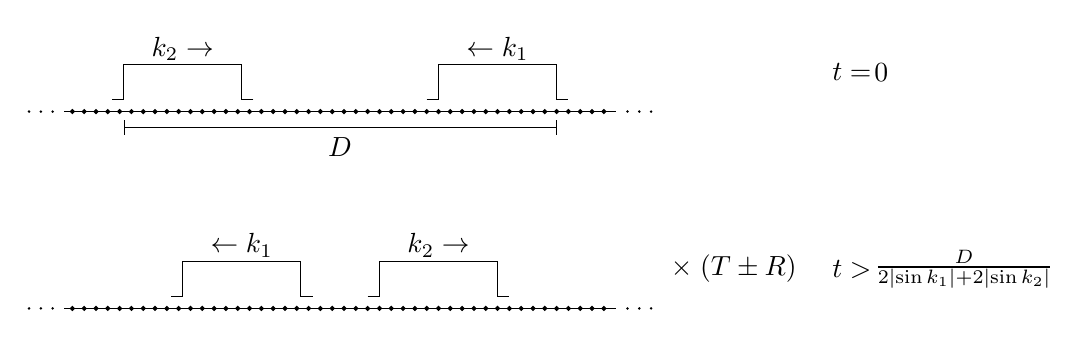
\begin{tikzpicture}[label distance= -6pt,
    verts/.style={circle,draw=black,fill=black,inner sep=.5pt,minimum size=0pt},
    dots/.style={circle,fill=black,inner sep=.25pt,minimum width=0pt}]
  \draw (0,0) -- (7,0);

  
  \draw (3.15,.15) -- (3,.15) -- (3,.6) -- (1.5,.6) 
     -- (1.5,.15) -- (1.35,.15);
  
  \draw (3.85,.15) -- (4,.15) -- (4,.6) -- (5.5,.6) 
     -- (5.5,.15) -- (5.65,.15);
     
  \node at (2.25,.8) {$\leftarrow k_1$};
  \node at (4.75,.8) {$k_2\rightarrow$};

  \node at (8.5,.5) {$\times \; (T\pm R)$};

  \node at (10,.5)[label=right:$\frac{D}{2|{\sin k_1}|+ 2|{\sin k_2}|}$]{$t>$};
  

  \foreach \x in {.1,.25,...,6.9}
  \node at (\x ,0) [verts] {};
  
  \begin{scope}[yshift=2.5cm]
    \draw (0,0) -- (7,0);

    \draw[xshift=-.75cm] (3.15,.15) -- (3,.15) -- (3,.6) -- (1.5,.6) 
       -- (1.5,.15) -- (1.35,.15);
  
    \draw[xshift=.75cm] (3.85,.15) -- (4,.15) -- (4,.6) -- (5.5,.6) 
       -- (5.5,.15) -- (5.65,.15);
 
    \draw [|-|] (.75,-.2) to node[below] {$D$} (6.25,-.2);
    
    \node at (1.5,.8) {$k_2\rightarrow$};
    \node at (5.5,.8) {$\leftarrow k_1$};

    \node at (10,.5)[label=right:$0$] {$t=$};

    \foreach \x in {.1,.25,...,6.9}
    \node at (\x ,0) [verts] {};

  \end{scope}

  \foreach \xsh in {-0.45cm, 7.15cm}{
  \foreach \ysh in {0cm, 2.5cm}{
    \begin{scope}[xshift=\xsh,yshift=\ysh]
      \node at (0,0) [dots]{};
      \node at (0.15,0) [dots] {};
      \node at (0.3,0) [dots]{};
    \end{scope}
  }}

\end{tikzpicture}
  \caption{Scattering of two particles on an infinite path.}
  \label{fig:wte}
\end{figure}


\subsection{Examples}

While our understanding of two-particle scattering for arbitrary interactions is useful, as we know that for almost any interaction the form of the eigenstates are scattering states, it will be useful to instantiate our claims and have explicit examples for the functions $\theta_{\pm}$.

\subsubsection{Bose-Hubbard model}

If we consider the Bose-Hubbard model for two particles, we have $\mathcal{V}(|r|) = \mathcal{U}_0^{2,2}\delta_{r,0}$. Here $C=0$ and $T=1+R$.  In this case the scattering state $|\mathrm{sc}(p_1;p_2)\rangle_+$ is
\begin{align}
\langle x,y|\mathrm{sc}(p_1;p_2)\rangle_+=\frac{1}{\sqrt{2}}e^{-ip_1 \left(\frac{x+y}{2}\right)}\left(e^{ip_2 |x-y|}+e^{i\theta_+(p_1,p_2)}e^{-ip_2 |x-y|}\right).
\end{align}
The first term describes the two particles moving toward each other and the second term describes them moving away from each other. To solve for the applied phase $e^{i\theta_+(p_1,p_2)}$ we look at the eigenvalue equation for $|\psi(p_1;p_2)\rangle$ at $r=0$. This gives
\begin{align}
  R(p_1,p_2) =- \frac{\mathcal{U}_0^{2,2}}{\mathcal{U}_0^{2,2} - 4i\cos({p_1}/{2})\sin(p_2)}.
\end{align}
So for the Bose-Hubbard model,
\begin{align}
  e^{i \theta_{+} (p_1,p_2)} = T(p_1,p_2) + R(p_1,p_2) = - \frac{ \mathcal{U}_0^{2,2} + 4 i \cos({p_1}/{2}) \sin(p_2)}{\mathcal{U}_0^{2,2} - 4 i \cos({p_1}/{2}) \sin(p_2)} =  \frac{2 \left(\sin(k_2) - \sin(k_1)\right) - i \mathcal{U}_0^{2,2}}{2 \left(\sin(k_2) - \sin(k_1)\right) + i \mathcal{U}_0^{2,2}}.
\end{align}
For example, if $\mathcal{U}_0^{2,2} = 2+\sqrt{2}$ then two particles with momenta $k_1 =-{ \pi}/{2}$ and $k_2={\pi}/{4}$ acquire a phase of $e^{-i\pi/2}= -i$ after scattering.

\subsubsection{Nearest-neighbor interaction}

%\todo{if time, find perfect reflection with good momenta}

For a multi-particle quantum walk with nearest-neighbor interactions, $\mathcal{V}(|r|)=\mathcal{U}_1^{1,1}\delta_{|r|,1}$ and $C=1$.  In this case the eigenvalue equations for $|\psi(p_1;p_2)\rangle$ at $r=-1$, $r=1$, and $r=0$ are
\begin{align}
 4 \cos\left(\frac{p_1}{2}\right)  \cos(p_2) ( e^{i p_2} + R(p_1,p_2) e^{-i p_2} ) &= U_1^{1,1} ( e^{i p_2} + R(p_1,p_2) e^{-i p_2}) \\
& \quad + 2\cos\left(\frac{p_1}{2}\right) \left( e^{2i p_2} + R(p_1,p_2) e^{-2i p_2}+f(p_1,p_2,0)\right) \\
 4 \cos\left(\frac{p_1}{2}\right)  \cos(p_2) T(p_1,p_2) e^{-ip_2} & =U_1^{1,1}T(p_1,p_2)e^{-ip_2}\\
& \quad +2\cos \left(\frac{p_1}{2}\right)\left(f(p_1,p_2,0)+T(p_1,p_2)e^{-2ip_2}\right)\\
2 \cos(p_2) f(p_1,p_2,0) &=T(p_1,p_2)e^{-ip_2}+e^{ip_2}+R(p_1,p_2)e^{-ip_2},
\end{align}
respectively.

Solving these equations for $R$, $T$, and $f(p_1,p_2,0)$, we can construct the corresponding scattering states for bosons, fermions, or distinguishable particles. Unlike the case of the Bose-Hubbard model, we may not have $1+R=T$. For example, when $U_1^{1,1}=-2-\sqrt{2}$, $p_1={\pi}/{4}$, and $p_2={3\pi}/{8}$, we get $R=0$ and $T=i$. 

Additionally, in the special case of $k_1 = \frac{2\pi}{3}$ and $k_2 = -\frac{\pi}{3}$, we have that 
\begin{align}
  R = \frac{U_1^{1,1}}{U_1^{1,1}-i \sqrt{3}} \qquad T = 1 - R = \frac{ \sqrt{3}}{\sqrt{3} + i U_1^{1,1}},
\end{align}
and thus $\theta_+(k_1,k_2) = 0$, while 
\begin{align}
  e^{i \theta_-(k_1,k_2)} = - \frac{U_1^{1,1} + i \sqrt{3}}{U_1^{1,1} - i \sqrt{3}}.
\end{align}
In this way, we have that the symmetric subspace has no acquired phase, while the anti-symmetric does acquire a phase.

\subsection{Two-particle orthonormality}

While the states $\ket{\mathrm{sc}(p_1;p_2)}$ do not necessarily span the entire Hilbert space, they will span the portion of the space that will be needed for this thesis.  However, we will need that they satisfy some orthogonality constraints, and in particular that they are (delta-function) orthonormal. As such, we have that the states $\{|\mathrm{sc}(p_1;p_2)\rangle \colon p_1\in (-\pi,\pi),\,p_2\in(-\pi,0)\cup(0,\pi)\}$ have the following inner product:
\begin{align}
\langle  \mathrm{sc}(p_1';p_2')|\mathrm{sc}(p_1;p_2)\rangle &= \langle \mathrm{sc}(p_1'; p_2')|\left(\sum_{\text{$r,s$ even}}|r\rangle\langle r| \otimes |s\rangle \langle s| \right)|\mathrm{sc}(p_1;p_2)\rangle\nonumber\\
&\qquad + \langle \mathrm{sc}(p_1'; p_2')|\left(\sum_{\text{$r,s$ odd}}|r\rangle \langle r|\otimes  |s\rangle \langle s|\right)|\mathrm{sc}(p_1;p_2)\rangle\\
&= \sum_{\text{$s$ even}} e^{-i(p_1-p_1') {s}/{2}}\sum_{\text{$r$ even}}\langle \psi(p_1';p_2')|r\rangle\langle r|\psi(p_1;p_2)\rangle\nonumber \\
& \qquad + \sum_{\text{$s$ odd}} e^{-i(p_1-p_1') {s}/{2}}\sum_{\text{$r$ odd}}\langle  \psi(p_1';p_2')|r\rangle\langle r|\psi(p_1;p_2)\rangle\\
&= 2\pi \delta(p_1-p_1') \sum_{r=-\infty}^{\infty}\langle \psi(p_1;p_2')|r\rangle\langle r|\psi(p_1;p_2)\rangle\\
&= 4\pi^2 \delta(p_1-p_1')\delta(p_2-p_2')
\end{align}
where in the last step we used the fact that $\langle\psi(p_1;p_2')|\psi(p_1;p_2)\rangle=2\pi\delta(p_2-p_2')$, which can be derived from \lem{orthonormality_of_scattering_states}.

%%%%%%%%%%%%%%%%%
%  Wave-packet scattering

\section{Wave-packet scattering}

Now that we have an understanding of the two-particle scattering eigenstates on an infinite path, we will want to understand the time-evolution of wave-packets on the infinite path.  In particular, if we initially have a product state corresponding to two wave-packets traveling towards each other, how does the time-evolved state look?

We would expect that the two wave-packets would simply evolve forward in time, where the center of the wave-packets each move with a speed $2\sin k_i$, possibly acquiring a phase if they move past each other.  It turns out that this is exactly what happens, but proving the fact is a little complicated. 

As this was a major component of \cite{MPQW}, a bound for this scattering behavior was proven using square wave-packets.
\begin{theorem}[Childs, Gosset, W \cite{MPQW}]Let $H^{(2)}$ be a two-particle Hamiltonian of the form \eq{MPQW_H_defn} with interaction range at most $d$, i.e., $\mathcal{V}(|r|)=0$ for all $|r|>d$. Let $\theta_{\pm}(p_1;p_2)$ be given by equation \eq{delta_pm}. Define $\theta=\theta_{\pm}({\pi}/{4},{3\pi}/{8})$. Let $L\in\NN$, let $M\in\{d+1,d+2,\ldots\}$, and define
\begin{align}
|\chi_{z,k}\rangle & =  \frac{1}{\sqrt{L}}\sum_{x=z-L}^{z-1}e^{ikx}|x\rangle\\
|\psi(0)\rangle & =  \frac{1}{\sqrt{2}}\left(|\chi_{-M,-\frac{\pi}{2}}\rangle|\chi_{M+L+1,\frac{\pi}{4}}\rangle 
	\pm |\chi_{M+L+1,\frac{\pi}{4}}\rangle|\chi_{-M,-\frac{\pi}{2}}\rangle\right).
\end{align}
Let $c_{0}$ be a constant independent of $L$. Then, for all $0\leq t\leq c_{0}L$, we have
\[
\left\Vert e^{-iH^{(2)}t}|\psi(0)\rangle-|\alpha(t)\rangle\right\Vert =\OO(L^{-{1}/{4}}),
\]
where 
\begin{equation}
|\alpha(t)\rangle=\sum_{x,y}a_{xy}(t)|x,y\rangle,
\end{equation}
$a_{xy}(t)=\pm a_{yx}(t)$ for $x \ne y$, and, for $x\leq y$, 
\begin{align}
a_{xy}(t) & =  \frac{1}{\sqrt{2}L}e^{-\sqrt{2}it}\left[e^{-i \pi x/2} e^{i \pi y/4} F(x,y,t) 
    \pm e^{i\theta} e^{i \pi x/4} e^{-i \pi y/2} F(y,x,t) \right]
\label{eq:a_xy}
\end{align}
where
\begin{align}
F(u,v,t) & =  \begin{cases}
	1 & \text{if }u-2 \lfloor t \rfloor\in\{-M-L,\ldots,-M-1\}\text{ and }v+2\left\lfloor \frac{t}{\sqrt{2}}
	\right\rfloor \in\{M+1,\ldots,M+L\}\\
	0 & \text{otherwise.}\end{cases}
\end{align}
\end{theorem}

Note that this was sufficient for their purposes, but the square wave-packets were most likely not optimal in terms of the resulting error.  In particular, one would expect something like a Gaussian wave-packet to have better error bounds.  

Along these lines, this section is focused on proving the following lemma discussing wave-packet propagation using Gaussian wave-packets:
%%%%%%%%%%%%%%%%%%%%%%%%%%%%%%%%%%%
\begin{theorem}
Let $H^{(2)}$ be a two-particle Hamiltonian of the form \eq{MPQW_H_defn} with interaction range at most $d$.  Let $\theta_{\pm}(p_1;p_2)$ be given by equation \eq{delta_pm} (with associated $\theta_{\pm}(k_1,k_2)$).  Let $k_1\in (-\pi,0)$ and let $k_2 \in (0,\pi)$, let $L,\mu, \nu \in \NN$ with $L>0$ and and let $\sigma > 0$.  Let us then define the states
\begin{align}
  \ket{\alpha(t)}_{\pm} = \frac{\gamma}{\sqrt{2}} e^{-2i t (\cos k_1 + \cos k_2)} \sum_{x = \mu(t)-L}^{\mu(t)+L} \sum_{y = \nu(t) -L}^{\nu(t)+L} e^{ -\frac{ (x-\mu(t))^2}{2\sigma^2} - \frac{(y-\nu(t))^2}{2\sigma^2}} e^{i k_1 x + i k_2 y} \alpha_{xy} \big( \ket{x,y} \pm \ket{y,x}\big),
\end{align}
where
\begin{align}
  \mu(t) = \mu - \lceil 2 t \sin k_1\rceil, \quad
  \nu(t) = \nu - \lceil 2 t \sin k_2\rceil, \qquad
  \alpha_{xy} = \begin{cases} 1  & y-x > r\\
  e^{i\theta_\pm(k_1,k_2)} & x-y > r\\
  0 & \text{otherwise},
  \end{cases}
\end{align}
and
\begin{align}
  \gamma^{-2} = \sum_{x,y=-L}^L e^{-\frac{1}{\sigma^2}(x^2+y^2)} = \Big(h_L^{\sigma/\sqrt{2}}(0)\Big)^2.
\end{align}
Additionally, let us define the initial state
\begin{align}
  \ket{\psi(0)}_{\pm} = \ket{\alpha(0)}_{\pm}.
\end{align}
If $\sigma = \frac{ L}{2\sqrt{\log L}}$, and if $0 \leq t < c L$ for some constant $c$, then 
\begin{align}
  \norm{e^{ - i H^2 t} \ket{\psi(0)}_{\pm} - \ket{\alpha(t)}}_{\pm} \leq 4 \sqrt{\frac{c\log L}{L}}.
\end{align}
\label{thm:two_particle_wave-packet_bound}
\end{theorem}

Note that we will use many of the tools used in the proof of \thm{single_particle_wavepacket_bound}, and in particular we use the function $h_L^\sigma(\phi)$ several times.

\begin{proof}
We will first want to show that our approximation to the time-evolved state is a nearly normalized state.  In particular, we have that
\begin{align}
  &{}_\pm\braket{\alpha(t)}{\alpha(t)}_\pm \nonumber\\
  &\qquad = \gamma^2 \Bigg[\sum_{x=\mu(t)-L}^{\mu(t)+L} \sum_{y=\nu(t)-L}^{\nu(t)+L} e^{-\frac{(x-\mu(t))^2}{\sigma^2} - \frac{(y-\nu(t))^2}{\sigma^2}} \nonumber\\
  &\qquad \qquad \pm  \sum_{x,y=\max\{\mu(t),\nu(t)\}-L}^{\min\{\mu(t),\nu(t)\}+L} e^{-\frac{(x-\mu(t))^2 + (x-\nu(t))^2 + (y-\mu(t))^2+(y-\nu(t))^2}{2\sigma^2}}e^{i (k_1-k_2) x}e^{i(k_2-k_1)y} \alpha_{xy}\alpha_{yx}^* \nonumber\\
  &\qquad \qquad - \sum_{x=\max\{\mu(t),\nu(t)\}-L}^{\min\{\mu(t),\nu(t)\}+L}\sum_{y=\max\{x-d,\mu(t)-L,\nu(t)-L\}}^{\min\{x+d,\mu(t)+L,\nu(t)+L\}} e^{-\frac{(x-\mu(t))^2}{\sigma^2} - \frac{(y-\nu(t))^2}{\sigma^2}} \Bigg].\label{eq:approximation_ip}
\end{align}
While this is a rather complicated expression when $|\mu(t) - \nu(t)| \leq 2L$, for times outside this range only the first term is nonzero, and is in fact exactly $\gamma^{-2}$.  Hence, for times when the two wave-packets do not overlap, our approximation $\ket{\alpha(t)}_{\pm}$ is exactly normalized.  If we can show that the latter two terms are small for all times $t$, we will then have that our approximation is almost normalized, as we need.

Let us first inspect the second term in \eq{approximation_ip}, corresponding to the cross terms between the two wave-packets.  We can expand the sum as
\begin{align}
  &\sum_{x,y=\max\{\mu(t),\nu(t)\}-L}^{\min\{\mu(t),\nu(t)\}+L} e^{-\frac{(x-\mu(t))^2 + (x-\nu(t))^2 + (y-\mu(t))^2+(y-\nu(t))^2}{2\sigma^2}}e^{i (k_1-k_2) x}e^{i(k_2-k_1)y} \alpha_{xy}\alpha_{yx}^*\nonumber\\
  &\qquad = e^{-i\theta_{\pm}} \sum_{\substack{x,y=\max\{\mu(t),\nu(t)\}-L\\y-x > d}}^{\min\{\mu(t),\nu(t)\}+L}  e^{-\frac{(x-\mu(t))^2 + (x-\nu(t))^2 + (y-\mu(t))^2+(y-\nu(t))^2}{2\sigma^2}} e^{i (k_1 - k_2) x}e^{i (k_2 - k_1) y}\nonumber\\
  &\qquad\qquad + e^{i\theta_{\pm}} \sum_{\substack{x,y=\max\{\mu(t),\nu(t)\}-L\\x-y > d}}^{\min\{\mu(t),\nu(t)\}+L}  e^{-\frac{(x-\mu(t))^2 + (x-\nu(t))^2 + (y-\mu(t))^2+(y-\nu(t))^2}{2\sigma^2}} e^{i (k_1 - k_2) x}e^{i (k_2 - k_1) y},
\end{align}
and then inspect each of these two terms individually.  We can then see
\begin{align}
 &\sum_{\substack{x,y=\max\{\mu(t),\nu(t)\}-L\\y-x > d}}^{\min\{\mu(t),\nu(t)\}+L}  e^{-\frac{(x-\mu(t))^2 + (x-\nu(t))^2 + (y-\mu(t))^2+(y-\nu(t))^2}{2\sigma^2}} e^{i (k_1 - k_2) x}e^{i (k_2 - k_1) y}\nonumber\\
 &\qquad = \sum_{x=\max\{\mu(t),\nu(t)\}-L}^{\min\{\mu(t),\nu(t)\}+L} e^{-\frac{(x-\mu(t))^2 + (x-\nu(t))^2}{2\sigma^2}} e^{i (k_1 - k_2) x}\sum_{y = x+d+1}^{\min\{\mu(t),\nu(t)\}+L} e^{-\frac{(y-\mu(t))^2+(y-\nu(t))^2}{2\sigma^2}} e^{i (k_2 - k_1) y}\\
 &\qquad = \sum_{x=\max\{\mu(t),\nu(t)\}-L}^{\min\{\mu(t),\nu(t)\}+L} e^{-\frac{(x-\mu(t))^2 + (x-\nu(t))^2}{2\sigma^2}} e^{i (k_1 - k_2) x} e^{-\frac{(\mu(t)-\nu(t))^2}{4\sigma^2}} \nonumber\\
 &\qquad \qquad \times\sum_{y=x+d+1}^{\min\{\mu(t),\nu(t)\}+L} e^{-\frac{(y - \frac{\mu(t)+\nu(t)}{2})^2}{\sigma^2}} e^{i (k_2-k_1)y}.\label{eq:diagonal_term_overlap_single}
\end{align}
Now, this second sum is simply a finite Gaussian approximation related to the $h$ function from \chap{scattering_on_graphs}, with an offset from the center.  From this, we have
\begin{align}
  &\sum_{y=x+d+1}^{\min\{\mu(t),\nu(t)\}+L} e^{-\frac{(y - \frac{\mu(t)+\nu(t)}{2})^2}{\sigma^2}} e^{i (k_2-k_1)y}= e^{i (k_2-k_1) \frac{\mu(t)+\nu(t)}{2}}\sum_{y = x+d+1 - \frac{\mu(t)+\nu(t)}{2}}^{\min\{\mu(t),\nu(t)\}+L - \frac{\mu(t)+\nu(t)}{2}} e^{ -\frac{y^2}{\sigma^2}} e^{i (k_2-k_1)y}.
\end{align}
Assuming that $\mu(t)+\nu(t)$ is even, this is simply
\begin{align}
   &e^{i (k_1 - k_2) \frac{\mu(t) + \nu(t)}{2}}\sum_{y=x+d+1}^{\min\{\mu(t),\nu(t)\}+L} e^{-\frac{(y - \frac{\mu(t)+\nu(t)}{2})^2}{\sigma^2}} e^{i (k_2-k_1)y}\nonumber\\
    &\qquad =\begin{cases} V_{1,\frac{\mu(t)+\nu(t)}{2} - x - d - 1}^{\frac{\sigma}{\sqrt{2}}}(k_1-k_2) + 1 + V_{1,L -\frac{ |\mu(t) - \nu(t)|}{2}}^{\frac{\sigma}{\sqrt{2}}}(k_2-k_1) & \mu(t) + \nu(t) > 2(x+d+1)\\
     V_{x+d+1-\frac{\nu(t)+\mu(t)}{2},L-\frac{|\nu(t)-\mu(t)|}{2}}^{\frac{\sigma}{\sqrt{2}}}(k_2-k_1) & \text{otherwise.}  
   \end{cases}\label{eq:overlap_y_sums}
\end{align}
For both cases, we have that this is bounded by some constant value in norm by \lem{tail_bounds} from \chap{scattering_on_graphs}.   If $\mu(t) + \nu(t)$ is odd, we can simply note that
\begin{align}
  \sum_{y=a}^b e^{-\frac{1}{\sigma^2}(y + \frac{1}{2})^2} e^{ i \phi y} &= e^{-i \frac{\phi}{2}} \sum_{y = a}^{b} e^{ - \frac{(2y + 1)^2}{4\sigma^2}} e^{ i \frac{\phi}{2} (2y + 1)}\\
  & = e^{ - i\frac{\phi}{2}} \Bigg[\sum_{z = 2a + 1}^{2b+1} e^{-\frac{z^2}{4\sigma^2} }e^{i \frac{\phi}{2} z}  - \sum_{z = a}^b e^{-\frac{z^2}{\sigma^2}} e^{i \phi z}\Bigg],
\end{align}
where both of the sums can be bounded by constants in norm in a manner similar to \eq{overlap_y_sums}.  As such, we have that for all times $t$,
\begin{align}
  \Bigg|\sum_{y =x+d+1}^{\min\{\mu(t),\nu(t)\} + L} e^{-\frac{(y-\frac{\mu(t)+\nu(t)}{2})^2}{\sigma^2}} e^{i (k_2-k_1)y} \Bigg| < \kappa
\end{align}
for some constant $\kappa$ that might depend on $L$, $\sigma$, and $k_2-k_1$.  We can then use this to bound the norm of \eq{diagonal_term_overlap_single} as
\begin{align}
  &\Bigg|\sum_{\substack{x,y=\max\{\mu(t),\nu(t)\}-L\\y-x > d}}^{\min\{\mu(t),\nu(t)\}+L}  e^{-\frac{(x-\mu(t))^2 + (x-\nu(t))^2 + (y-\mu(t))^2+(y-\nu(t))^2}{2\sigma^2}} e^{i (k_1 - k_2) x}e^{i (k_2 - k_1) y}\Bigg|\nonumber\\
  &\qquad \leq \kappa e^{- \frac{(\mu(t) - \nu(t))^2}{2\sigma^2}} \sum_{x=\max\{\mu(t),\nu(t) \}-L}^{\min\{\mu(t),\nu(t)\}+L} e^{ - \frac{\big( x - \frac{\mu(t) + \nu(t)}{2}\big)^2}{\sigma^2}}\\
  &\qquad \leq \kappa e^{-\frac{(\mu(t)-\nu(t))^2}{2\sigma^2}} h_{\infty}^{\sqrt{2}\sigma}(0)\\
  &\qquad \leq 6\sqrt{\pi} \sigma \kappa e^{-\frac{(\mu(t)-\nu(t))^2}{2\sigma^2}},
\end{align}
where the second inequality arose since we didn't know whether $\mu(t)+\nu(t)$ was even or odd, and the third from our bounds on $h_{\infty}^\sigma(0)$.  A similar argument gives the same bound for the sum with $x-y > d$.

For the third term in \eq{approximation_ip}, we again use a rather simple approximation.  Namely, we have
\begin{align}
  \sum_{x=\max\{\mu(t),\nu(t)\}-L}^{\min\{\mu(t),\nu(t)\}+L}\sum_{y=\max\{x-d,\mu(t)-L,\nu(t)-L\}}^{\min\{x+d,\mu(t)+L,\nu(t)+L\}} e^{-\frac{(x-\mu(t))^2}{\sigma^2} - \frac{(y-\nu(t))^2}{\sigma^2}} &< (2d+1) h_\infty^{\sigma/\sqrt{2}} (0)\\
  & < (2d+1) 2\sqrt{\pi} \sigma ,
\end{align}
where we again used our bounds on $h_\infty^\sigma(0)$ from \lem{h_bounds} from \chap{scattering_on_graphs}.

Putting these bounds together, we then have that
\begin{align}
  &\Big|{}_\pm\braket{\alpha(t)}{\alpha(t)}_{\pm} - 1 \Big| \nonumber\\
  & \qquad\leq \gamma^2 \Bigg[ \Bigg|\sum_{x,y=\max\{\mu(t),\nu(t)\}-L}^{\min\{\mu(t),\nu(t)\}+L} e^{-\frac{(x-\mu(t))^2 + (x-\nu(t))^2 + (y-\mu(t))^2+(y-\nu(t))^2}{2\sigma^2}}e^{i (k_1-k_2) x}e^{i(k_2-k_1)y} \alpha_{xy}\alpha_{yx}^*\Bigg| \nonumber\\
  &\qquad \qquad + \Bigg|\sum_{x=\max\{\mu(t),\nu(t)\}-L}^{\min\{\mu(t),\nu(t)\}+L}\sum_{y=\max\{x-d,\mu(t)-L,\nu(t)-L\}}^{\min\{x+d,\mu(t)+L,\nu(t)+L\}} e^{-\frac{(x-\mu(t))^2}{\sigma^2} - \frac{(y-\nu(t))^2}{\sigma^2}} \Bigg|\Bigg]\\
  &\qquad \leq  \gamma^2 \Bigg[2 \bigg(6 \sqrt{\pi} \sigma \kappa e^{-\frac{(\mu(t)-\nu(t))^2}{2\sigma^2}} \bigg) + 2(2d+1)\sqrt{\pi} \sigma \Bigg]\\
  &\qquad \leq 2\sqrt{\pi} \sigma \gamma^2 \big(\kappa + 2d + 1 \big).
\end{align}
Since $\gamma^2\propto \sigma^{-2}$, we then have that our normalization is then off by something bounded by $\OO(\sigma^{-1})$, which will be sufficient for our purposes.


With the above bounds on the normalization, we can now analyze our approximations to the time-evolved states. We find that 
\begin{align}
  &{}_{\pm}\braket{\scat(p_1;p_2)}{\alpha(t)}_\pm \nonumber\\
  &\qquad= \frac{\gamma e^{-2it(\cos(k_1) + \cos(k_2))}}{\sqrt{2}} \sum_{x= \mu(t) -L}^{\mu(t) + L} \sum_{y=\nu(t) -L}^{\nu(t)+L} e^{i k_1 x} e^{i k_2 y} e^{-\frac{(x-\mu(t))^2}{2\sigma^2}} e^{-\frac{(y-\nu(t))^2}{2\sigma^2}} \beta_{x,y}\nonumber\\
  &\qquad\qquad\times\Big({}_{\pm}\braket{\scat(p_1;p_2)}{x,y} \pm  {}_{\pm}\braket{\scat(p_1;p_2)}{y,x}\Big)\\
  &\qquad = \gamma e^{-2it(\cos(k_1) + \cos(k_2))} \sum_{x=\mu(t)-L}^{\mu(t)+L} \sum_{\substack{y=\nu(t)-L\\y > x+r}}^{\nu(t)+L}  e^{i k_1 x} e^{i k_2 y} e^{-\frac{(x-\mu(t))^2}{2\sigma^2}} e^{-\frac{(y-\nu(t))^2}{2\sigma^2}} \nonumber\\
  &\qquad\qquad\times e^{i \frac{p_1}{2} (x+y)}\Big(e^{i p_2 (x-y)} \pm e^{-i\theta_{\pm}(p_1;p_2)} e^{- i p_2 (x-y)}\Big)\nonumber\\
  &\qquad \qquad+ \gamma e^{-2it(\cos(k_1) + \cos(k_2))} \sum_{x=\mu(t)-L}^{\mu(t)+L} \sum_{\substack{y=\nu(t)-L\\y < x-r}}^{\nu(t)+L}  e^{i k_1 x} e^{i k_2 y} e^{-\frac{(x-\mu(t))^2}{2\sigma^2}} e^{-\frac{(y-\nu(t))^2}{2\sigma^2}}e^{i\theta_{\pm}(k_1,k_2)} \nonumber\\
  &\qquad\qquad\times e^{i \frac{p_1}{2} (x+y)}\Big(e^{-i\theta_\pm(p_1;p_2)} e^{i p_2 (x-y)} \pm  e^{- i p_2 (x-y)}\Big).
\end{align}
While this is a rather complicated expression, if we break the terms into smaller pieces, we find that
\begin{align}
  &{}_{\pm}\braket{\scat(p_1;p_2)}{\alpha(t)}_\pm \nonumber\\
  &\qquad = \gamma e^{-2i t (\cos(k_1) + \cos (k_2))}\Bigg[\sum_{x=\mu(t)-L}^{\mu(t)+L} \sum_{\substack{y=\nu(t)-L\\y > x+r}}^{\nu(t)+L} e^{-\frac{(x-\mu(t))^2}{2\sigma} - \frac{(y-\nu(t))^2}{2\sigma^2}} e^{i \big(\frac{k_1 + k_2}{2} +\frac{p_1}{2} \big)(x+y)}\nonumber\\
  &\qquad\qquad \times\Big( e^{i \big(\frac{k_1 - k_2}{2} + p_2 \big) (x-y)} \pm e^{-i\theta_{\pm}(p_1;p_2)} e^{i \big(\frac{k_1-k_2}{2} - p_2 \big)(x-y)} \Big) \nonumber\\
  &\qquad\qquad+\sum_{x=\mu(t)-L}^{\mu(t)+L} \sum_{\substack{y=\nu(t)-L\\y < x-r}}^{\nu(t)+L} e^{-\frac{(x-\mu(t))^2}{2\sigma} - \frac{(y-\nu(t))^2}{2\sigma^2}} e^{i \big(\frac{k_1 + k_2}{2} +\frac{p_1}{2} \big)(x+y)}\nonumber\\
  &\qquad\qquad \times\Big(e^{i\big(\theta_{\pm}(k_1,k_2) - \theta_\pm(p_1;p_2)\big)} e^{i \big(\frac{k_1 - k_2}{2} + p_2 \big) (x-y)} \pm  e^{i\theta_{\pm}(k_1,k_2) }e^{i (\frac{k_1-k_2}{2} - p_2 )(x-y)} \Big)\Bigg]\\
  &\qquad = \gamma e^{-2it (\cos(k_1) + \cos(k_2))} \Bigg[ \sum_{x=\mu(t)-L}^{\mu(t)+L} \sum_{y=\nu(t)-L}^{\nu(t)+L} e^{-\frac{(x-\mu(t))^2}{2\sigma^2} - \frac{(y-\nu(t))^2}{2\sigma^2}} e^{i (k_1 + \frac{p_1}{2} + p_2)x}e^{i(k_2 + \frac{p_1}{2} - p_2)y} \nonumber\\ 
  &\qquad\qquad + \Big(e^{i(\theta_{\pm}(k_1,k_2) - \theta_{\pm}(p_1;p_2))} - 1\Big)\nonumber\\
  &\qquad\qquad\qquad\times\sum_{x=\mu(t)-L}^{\mu(t)+L} \sum_{\substack{y=\nu(t)-L\\y>x+r}}^{\nu(t)+L} e^{-\frac{(x-\mu(t))^2}{2\sigma^2} - \frac{(y-\nu(t))^2}{2\sigma^2}} e^{i (k_1 + \frac{p_1}{2} + p_2)x}e^{i(k_2 + \frac{p_1}{2} - p_2)y}\nonumber\\
  &\qquad\qquad \pm \Big(e^{-i\theta_{\pm}(p_1;p_2)}\delta_{\mu(t)\leq\nu(t)} + e^{i  \theta_{\pm}(k_1,k_2)}\delta_{\mu(t) > \nu(t)}\Big)\nonumber\\
  &\qquad\qquad\qquad\times\sum_{x=\mu(t)-L}^{\mu(t)+L} \sum_{y=\nu(t)-L}^{\nu(t)+L} e^{-\frac{(x-\mu(t))^2}{2\sigma^2} - \frac{(y-\nu(t))^2}{2\sigma^2}} e^{i (k_1 + \frac{p_1}{2} - p_2)x}e^{i(k_2 + \frac{p_1}{2} + p_2)y}\nonumber\\
  &\qquad\qquad \pm \delta_{\mu(t)\leq \nu(t)} \big( e^{i\theta_{\pm}(k_1,k_2)} - e^{-i\theta_{\pm}(p_1;p_2)}\big)\nonumber\\
  &\qquad\qquad\qquad\times\sum_{x=\mu(t)-L}^{\mu(t)+L} \sum_{\substack{y=\nu(t)-L\\y< x-r}}^{\nu(t)+L} e^{-\frac{(x-\mu(t))^2}{2\sigma} - \frac{(y-\nu(t))^2}{2\sigma^2}} e^{i (k_1 + \frac{p_1}{2} - p_2)x}e^{i(k_2 + \frac{p_1}{2} + p_2)y}\nonumber\\
  &\qquad\qquad \pm \delta_{\mu(t)> \nu(t)} \big( e^{-i\theta_{\pm}(p_1;p_2)} - e^{i\theta_{\pm}(k_1,k_2)}\big)\nonumber\\
  &\qquad\qquad\qquad\times\sum_{x=\mu(t)-L}^{\mu(t)+L} \sum_{\substack{y=\nu(t)-L\\y> x+r}}^{\nu(t)+L} e^{-\frac{(x-\mu(t))^2}{2\sigma} - \frac{(y-\nu(t))^2}{2\sigma^2}} e^{i (k_1 + \frac{p_1}{2} - p_2)x}e^{i(k_2 + \frac{p_1}{2} + p_2)y}\nonumber\\
  &\qquad\qquad -\sum_{x=\mu(t)-L}^{\mu(t)+L} \sum_{\substack{y=\nu(t)-L\\|x-y|\leq r}}^{\nu(t)+L} e^{-\frac{(x-\mu(t))^2}{2\sigma} - \frac{(y-\nu(t))^2}{2\sigma^2}}\bigg( e^{i (k_1 + \frac{p_1}{2} + p_2)x}e^{i(k_2 + \frac{p_1}{2} - p_2)y} \nonumber\\
  &\qquad\qquad \pm \Big(e^{-i\theta_{\pm}(p_1;p_2)}\delta_{\mu(t)\leq\nu(t)} + e^{i  \theta_{\pm}(k_1,k_2)}\delta_{\mu(t) > \nu(t)}\Big) e^{i (k_1 + \frac{p_1}{2} - p_2)x}e^{i(k_2 + \frac{p_1}{2} + p_2)y}\bigg)\Bigg].\label{eq:alpha_scat_ip}
\end{align}
While this expansion takes up much more room than before, it nicely organizes each of the terms in the inner product.  Depending on the value of $p_1$ and $p_2$, most of the norm in \eq{alpha_scat_ip} is on either the first or the third terms, with the rest small corrections.  In fact, the first of these terms is proportional to $h_{L}^\sigma (k_1+p_1/2 + p_2) h_L^\sigma(k_2+p_1/2- p_2)$, while the second is similar but with $p_2\mapsto -p_2$.

With a decent understanding of these inner products, we can now define a Gaussian approximation to our assumed approximation of the time-evolved states.  In particular, since most of the norm is contained on terms proportional to a product of $h_L^\sigma(\theta)$, our approximated time-evolved states will be centered about those $p_1$ and $p_2$ such that the $\theta \approx 0$.  Explicitly, let us then define the states
\begin{align}
  \ket{w(t)} &= \eta e^{ - 2 i t (\cos k_1 + \cos k_2)} \int_{-\delta}^\delta \int_{-\delta}^\delta \frac{d\phi_1 d\phi_2}{4\pi^2} e^{i \phi_1 \big(\frac{\mu(t) + \nu(t)}{2}\big)} e^{i  \phi_2 (\mu(t) - \nu(t))} \nonumber\\
  &\qquad\qquad \times e^{ -\frac{ \sigma^2 \phi_1^2}{4}} e^{ -\sigma^2 \phi_2^2} \ket{\scat(p_1 + \phi_1; p_2 + \phi_2)}_{\pm}
\end{align} 
where
\begin{align}
p_1 &= - k_1 - k_2 & p_2 & = \frac{k_2 - k_1}{2} &
  \eta^{-2} &= \int_{-\infty}^\infty \int_{-\infty}^\infty \frac{d\phi_1 d\phi_2}{4\pi^2} e^{ -\sigma^2 \big(\frac{\phi_1^2}{2} + 2 \phi_2^2 \big)} = \frac{1}{4\pi\sigma^2},
\end{align}
and $\delta$ is a constant that we will define later.  While the states $\ket{w(t)}$ are not exactly normalized, we have that
\begin{align}
   \braket{w(t)}{w(t)} &= \eta^2 \int_{-\delta}^\delta \int_{-\delta}^\delta \frac{d\phi_1d\phi_2}{4\pi^2}  e^{ -\sigma^2 \big(\frac{\phi_1^2}{2} + 2 \phi_2^2 \big)} &= 1  - \frac{\eta^2}{\pi^2} \int_\delta^{\infty} \int_{\delta}^\infty d\phi_1d\phi_2 e^{ - \sigma^2 \big(\frac{\phi_1^2}{2} + 2 \phi_2^2\big)}\label{eq:w_norm}\\
   & \geq  1 - \frac{1}{\pi \delta^2 \sigma^2}e^{- \frac{5 \sigma^2 \delta^2}{2}},
\end{align}
and as the second term on the right hand side of \eq{w_norm} is non-negative, we have that $\braket{w(t)}{w(t)} \leq 1$.

%%%%
% 1 integrand

We will now want to understand the relationship between the $\ket{\alpha(t)}$ and $\ket{w(t)}$, as we did in the proof of \thm{single_particle_wavepacket_bound}.  We then have
\begin{align}
&\braket{w(t)}{\alpha(t)}_{\pm} \nonumber\\
&\qquad = \eta e^{2it(\cos k_1 + \cos k_2)}\int_{-\delta}^\delta \frac{d\phi_1 d\phi_2}{4\pi^2} e^{-i \phi_1 \frac{\mu(t) + \nu(t)}{2}} e^{i \phi_1(\nu(t) - \mu(t))} e^{-\frac{\sigma^2 \phi_1^2}{4} - \sigma^2 \phi_2^2}\nonumber\\
&\qquad\qquad\qquad\qquad {}_\pm\braket{\scat(p_1+\phi_1;p_2+\phi_2)}{\alpha(t)}_\pm.\label{eq:w_alpha_ip}
\end{align}
It will then be worthwhile to expand ${}_\pm\braket{\scat(p_1+\phi_2;p_2+\phi_2)}{\alpha(t)}_\pm$ as in \eq{alpha_scat_ip}, and bound the norm for each term individually.   By contracting terms and by a slight relabelling of the dummy variable used for the sums, we then have the first term in the integrand for \eq{w_alpha_ip} is exactly
\begin{align}
  &\iint_{-\delta}^\delta \frac{d\phi_1 d\phi_2}{4\pi^2}e^{-\frac{\sigma^2\phi_1^2}{2} - \sigma^2 \phi_2^2} h_L^\sigma\Big(\frac{\phi_1}{2} + \phi_2\Big)h_L^\sigma\Big(\frac{\phi_1}{2} - \phi_2\Big)\\
  &\qquad = \iint_{-\delta}^\delta \frac{d\phi_1 d\phi_2}{4\pi^2}e^{-\frac{\sigma^2\phi_1^2}{2} - \sigma^2 \phi_2^2} \bigg[h_\infty^\sigma\Big(\frac{\phi_1}{2} + \phi_2\Big)h_\infty^\sigma\Big(\frac{\phi_1}{2} - \phi_2\Big)\nonumber\\
  &\qquad\qquad + h_\infty^\sigma\Big(\frac{\phi_1}{2} + \phi_2\Big)\bigg[h_L^\sigma\Big(\frac{\phi_1}{2} - \phi_2\Big) - h_\infty^\sigma\Big(\frac{\phi_1}{2} - \phi_2\Big)\bigg]\nonumber\\
  &\qquad\qquad + \bigg[h_L^\sigma\Big(\frac{\phi_1}{2} + \phi_2\Big) - h_\infty^\sigma\Big(\frac{\phi_1}{2} + \phi_2\Big)\bigg]h_L^\sigma\Big(\frac{\phi_1}{2} - \phi_2\Big)\bigg]\label{eq:w_alpha_important}.
\end{align}
Again, there are several integrals, but most of the amplitude is contained on the first.  For the first term, we can actually show that the integral is at least
\begin{align}
  &\int_{-\delta}^\delta \int_{-\delta}^{\delta} \frac{ d\phi_1 d\phi_2}{4\pi^2} e^{ - \frac{\sigma^2\phi_1^2}{4} - \sigma^2 \phi_2^2} h_\infty^\sigma \Big(\frac{\phi_1}{2} - \phi_2\Big) h_\infty^\sigma \Big( \frac{\phi_1}{2} + \phi_2\Big)\nonumber\\
  & \qquad =  \frac{\sigma^2}{2\pi} \int_{-\delta}^\delta \int_{-\delta}^\delta d\phi_1 d\phi_2 e^{ -\frac{\sigma^2 \phi_1^2}{2} - 2\sigma^2 \phi_2^2} h_\infty^{1/(2\pi \sigma)} \Big[2 \pi i \sigma^2 \Big(\frac{\phi_1}{2} - \phi_2 \Big)\Big]h_\infty^{1/(2\pi \sigma)} \Big[2 \pi i \sigma^2 \Big(\frac{\phi_1}{2} +\phi_2 \Big)\Big]\\
 & \qquad \geq \frac{\sigma^2}{2\pi} \int_{-\delta}^\delta \int_{-\delta}^\delta d\phi_1 d\phi_2 e^{ -\frac{\sigma^2 \phi_1^2}{2} - 2\sigma^2 \phi_2^2}\\
 & \qquad = \frac{1}{2} \braket{w(t)}{w(t)}
\end{align}
where we used the fact that $h_\infty^\sigma(i \phi) \geq 1$ for real $\phi$.  Using the upper bounds on $h$ from \lem{h_bounds}, we also have that
\begin{align}
&\int_{-\delta}^\delta \int_{-\delta}^{\delta} \frac{ d\phi_1 d\phi_2}{4\pi^2} e^{ - \frac{\sigma^2\phi_1^2}{4} - \sigma^2 \phi_2^2} h_\infty^\sigma \Big(\frac{\phi_1}{2} - \phi_2\Big) h_\infty^\sigma \Big( \frac{\phi_1}{2} + \phi_2\Big)\nonumber\\
& \qquad \leq \frac{\sigma^2}{2\pi} \int_{-\delta}^\delta \int_{-\delta}^\delta d\phi_1 d\phi_2 e^{ -\frac{\sigma^2 \phi_1^2}{2} - 2\sigma^2 \phi_2^2} \Bigg[1 + 2 \Big(1 + \frac{ 1}{\pi \sigma^2} \frac{1}{4 \pi -  | \phi_1 - 2\phi_2|} \Big)e^{-2\pi^2 \sigma^2 + \pi \sigma^2 (\phi_1 - 2 \phi_2)} \Bigg]\nonumber\\
& \qquad \qquad \times   \Bigg[1 + 2 \Big(1 + \frac{ 1}{\pi \sigma^2} \frac{1}{4 \pi -  | \phi_1+ 2\phi_2|} \ \Big)e^{-2\pi^2 \sigma^2 +   \pi \sigma^2 (\phi_1 + 2 \phi_2)} \Bigg]\\
& \qquad \leq \frac{1}{2} \Big[1 + 3 e^{ -  \pi^2 \sigma^2 \big(2 \pi - 3\delta\big)} \Big]^2  \braket{w(t)}{w(t)}
\end{align}
where we assumed that $2\pi > 3 \delta$, and that $\sigma \geq 1$. 

For the second and third terms of \eq{w_alpha_important}, note that for any real $\varphi_1$, $\varphi_2$, and for any $L_1,L_2 > \sigma \geq 1$, we have that
\begin{align}
  &\Big| h_{L_1}^\sigma(\varphi_1) \big(h_{L_2}^\sigma(\varphi_2) - h_\infty^\sigma(\varphi_2) \big) \Big| \nonumber\\
  &\qquad\leq \big| h_\infty^\sigma(0)\big| \frac{2\sigma^2}{L_2} e^{-\frac{L_2^2}{2\sigma^2}}\\
   & \qquad \leq  \frac{2 \sigma^2}{L} e^{-\frac{L^2}{2\sigma^2} }\Big [ 1 + 2 (1 + \sigma^2) e^{ -\frac{1}{2\sigma^2}}\Big]\\
   & \qquad \leq \frac{6 \sigma^4}{L}  e^{ - \frac{L^2}{2\sigma^2}}.
\end{align}
If we then use this bound for both of the integrands, we have 
\begin{align}
  &\Bigg | \int_{-\delta}^\delta \int_{-\delta}^\delta \frac{d\phi_1 d\phi_2}{4\pi^2} e^{- \frac{\sigma^2 \phi_1^2}{4}}e^{-\sigma^2 \phi_2^2}  \Big[h_\infty^\sigma\Big(\frac{\phi_1}{2} + \phi_2\Big)\bigg[h_L^\sigma\Big(\frac{\phi_1}{2} - \phi_2\Big) - h_\infty^\sigma\Big(\frac{\phi_1}{2} - \phi_2\Big)\bigg]\nonumber\\
  &\qquad + \bigg[h_L^\sigma\Big(\frac{\phi_1}{2} + \phi_2\Big) - h_\infty^\sigma\Big(\frac{\phi_1}{2} + \phi_2\Big)\bigg]h_L^\sigma\Big(\frac{\phi_1}{2} - \phi_2\Big)\bigg]\Bigg|\nonumber\\
  &\qquad \qquad \leq  2\int_{-\delta}^\delta \int_{-\delta}^\delta \frac{d\phi_1 d\phi_2}{4\pi^2} e^{- \frac{\sigma^2 \phi_1^2}{4}}e^{-\sigma^2 \phi_2^2}  \frac{6 \sigma^4}{L}  e^{-\frac{L^2}{2\sigma^2}}\\
  & \qquad\qquad < \frac{3\sigma^4}{\pi^2 L}  e^{ - \frac{ L^2}{2\sigma^2}}\int_{-\infty}^\infty \int_{-\infty}^\infty  d\phi_1 d\phi_2 e^{- \frac{\sigma^2 \phi_1^2}{4}}e^{-\sigma^2 \phi_2^2}\\
  & \qquad\qquad = \frac{ 6\sigma^2}{\pi L}  e^{ - \frac{L^2}{2\sigma^2}}.
\end{align}
From this, we then approximately know the norm of the first term in \eq{w_alpha_ip}.

%%
% Second integrand
For the second term in \eq{w_alpha_ip}, we will show that it can be bounded in norm, using the fact that the angle $\theta_\pm(p_1,p_2)$ is a bounded rational function of the momentum.  From this, we know that it is differentiable as a function of both $\phi_1$ and $\phi_2$ on some neighborhood $U$ of $(p_1,p_2)$.  Let us assume that $\delta$ is chosen so that $[-\delta,\delta]\times [-\delta,\delta] \subset U$, and now let
\begin{align}
  \Gamma = \max_{[-\delta,\delta]\times [-\delta,\delta]} \big|\nabla e^{i \theta_{\pm}(p_1 +\phi_1, p_2 +\phi_2)}\big|.
\end{align}
  We then have that
\begin{align}
  &\Bigg| \iint_{-\delta}^\delta \frac{d\phi_1d\phi_2}{4\pi^2} e^{-i \phi_1 \frac{\mu(t) + \nu(t)}{2}} e^{i \phi_1(\nu(t) - \mu(t))} e^{-\frac{\sigma^2 \phi_1^2}{4} - \sigma^2 \phi_2^2} \nonumber\\
  & \qquad \times \Big(e^{i(\theta_{\pm}(k_1,k_2) - \theta_{\pm}(p_1;p_2))} - 1\Big)\sum_{x=\mu(t)-L}^{\mu(t)+L} \sum_{\substack{y=\nu(t)-L\\y>x+r}}^{\nu(t)+L} e^{-\frac{(x-\mu(t))^2}{2\sigma^2} - \frac{(y-\nu(t))^2}{2\sigma^2}} e^{i (k_1 + \frac{p_1}{2} + p_2)x}e^{i(k_2 + \frac{p_1}{2} - p_2)y} \Bigg|\nonumber\\
  &\qquad \qquad < \iint_{-\delta}^\delta \frac{d\phi_1d\phi_2}{4\pi^2} \Gamma \sqrt{\phi_1^2 +\phi_2^2} e^{-\frac{\sigma^2 \phi_1^2}{4} - \sigma^2 \phi_2^2}h_L^\sigma (0) h_L^\sigma(0)\\
  &\qquad \qquad < \frac{\Gamma\sigma^2}{2\pi} \iint_{-\infty}^\infty d\phi_1 d\phi_2 \sqrt{\phi_1^2 + \phi_2^2} e^{-\frac{\sigma^2}{4} (\phi_1^2 + \phi_2^2)}\\
  &\qquad \qquad = \Gamma\sigma^2 \int_{0}^\infty r^2 e^{-\frac{\sigma^2}{4}r^2} dr\\
  &\qquad \qquad = \frac{2\sqrt{\pi}\Gamma}{\sigma}
\end{align}
and we have a bound on the norm of the second term in \eq{w_alpha_ip}.

%%
% third integrand
The third term in \eq{w_alpha_ip} is bound in a manner very similar to the first term. In particular, can rearrange the sums, so that the term is proportional to the product of two $h_L^\sigma(\theta)$, where the $\theta$ is bounded away from 0.  If we take the absolute value, so as to get rid of the extraneous phases, we find that
\begin{align}
&\Bigg| \int_{-\delta}^\delta \int_{-\delta}^{\delta} \frac{ d\phi_1 d\phi_2}{4\pi^2} e^{ - \frac{\sigma^2\phi_1^2}{4} - \sigma^2 \phi_2^2} \Big(e^{-i\theta_{\pm}(p_1;p_2)}\delta_{\mu(t)\leq\nu(t)} + e^{i  \theta_{\pm}(k_1,k_2)}\delta_{\mu(t) > \nu(t)}\Big) \nonumber\\
&\qquad e^{i (k_1-k_2  - 2\phi_2)\mu(t)}e^{i(k_2 -k_1 +2\phi_2)\nu(t)}h_L^\sigma \Big(k_1 -k_2 +\frac{\phi_1}{2} - \phi_2\Big) h_L^\sigma \Big(k_2 - k_1 + \frac{\phi_1}{2} + \phi_2\Big)\Bigg|\nonumber\\
&\qquad \qquad \leq \iint_{-\delta}^\delta \frac{d\phi_1d\phi_2}{4\pi^2} e^{ - \frac{\sigma^2\phi_1^2}{4} - \sigma^2 \phi_2^2}\bigg| h_L^\sigma \Big(k_1 -k_2 +\frac{\phi_1}{2} - \phi_2\Big) h_L^\sigma \Big(k_2 - k_1 + \frac{\phi_1}{2} + \phi_2\Big)\bigg|.
\end{align}
If we then approximate the $h_L$ by $h_\sigma$, as we did for the first term, we can use the exact same bound for the difference, as there was no reliance on the arguments to the $h$ functions, other than that they were purely real.  As such, we need only bound the above integral for infinite $h$'s.
\begin{align}
&\iint_{-\delta}^\delta \frac{d\phi_1d\phi_2}{4\pi^2} e^{ - \frac{\sigma^2\phi_1^2}{4} - \sigma^2 \phi_2^2}\bigg| h_\infty^\sigma \Big(k_1 -k_2 +\frac{\phi_1}{2} - \phi_2\Big) h_\infty^\sigma \Big(k_2 - k_1 + \frac{\phi_1}{2} + \phi_2\Big)\bigg|\nonumber\\
&\qquad \leq \frac{\sigma^2}{2\pi} \iint_{-\delta}^\delta e^{-\sigma^2\big( \frac{\phi_1^2}{2}  + \phi_2^2 + \big( \phi_2 + k_1-k_2\big)^2\big)} \nonumber\\
&\qquad\qquad\times h_{\infty}^{1/(2\pi\sigma)} \Big[2\pi i \sigma^2 \Big(k_2 - k_1 + \frac{\phi_1}{2} +\phi_2 \Big)\Big] h_\infty^{1/(2\pi\sigma)}\Big[ 2\pi i \sigma^2  \Big(k_1 - k_2+ \frac{\phi_1}{2}  -\phi_2 \Big) \Big]\\
    & \qquad\leq  \frac{\sigma^2}{2\pi}\int_{-\delta}^\delta \int_{-\delta}^\delta {d\phi_1 d\phi_2}  e^{- \frac{\sigma^2 \phi_1^2}{2}}e^{-\sigma^2 (\phi_2^2 + (2p_2 + \phi_2)^2)}\nonumber\\
    &\qquad\qquad \times\big( 1 + 3 e^{ - 2 \pi \sigma^2 ( \pi - | 2 p_2 + \phi_2 - \frac{\phi_1}{2} | )}\big) \big( 1 + 3 e^{ - 2 \pi \sigma^2 ( \pi - | 2 p_2 + \phi_2 + \frac{\phi_1}{2} | )}\big) 
\end{align}
At this point, if $\pi > |k_1-k_2|$, we can choose $\delta$ so that $\pi > |k_1-k_2| + 2\delta$ and thus 
\begin{align}
 &\iint_{-\delta}^\delta \frac{d\phi_1d\phi_2}{4\pi^2} e^{ - \frac{\sigma^2\phi_1^2}{4} - \sigma^2 \phi_2^2}\bigg| h_\infty^\sigma \Big(k_1 -k_2 +\frac{\phi_1}{2} - \phi_2\Big) h_\infty^\sigma \Big(k_2 - k_1 + \frac{\phi_1}{2} + \phi_2\Big)\bigg|\nonumber\\
&\qquad \leq \frac{2\sigma^2}{\pi}\int_{-\delta}^\delta \int_{-\delta}^\delta {d\phi_1 d\phi_2}  e^{- \sigma^2 \phi_1^2}e^{-\sigma^2 (\phi_2^2 + (2p_2 + \phi_2)^2)}\\
    & \qquad \leq \frac{2 \sigma}{\sqrt{\pi}} \int_{-\delta}^\delta d\phi_2 e^{ - 2\sigma^2 ( p_2^2 + (p_2 + \phi_2)^2)}\\
    &\qquad \leq 4\sqrt{2} e^{ -2 \sigma^2 p_2^2} = 4\sqrt{2} e^{-\frac{\sigma^2}{2} (k_2-k_1)^2}.
\end{align}
However, if $\pi \leq |k_1 -k_2|$, we can instead bound the functions approximating $h$ by their largest value, which is attained when $2\phi_2 \pm \phi_1 = 3 \delta$.  In particular, we have
\begin{align}
    &\iint_{-\delta}^\delta \frac{d\phi_1d\phi_2}{4\pi^2} e^{ - \frac{\sigma^2\phi_1^2}{4} - \sigma^2 \phi_2^2}\bigg| h_\infty^\sigma \Big(k_1 -k_2 +\frac{\phi_1}{2} - \phi_2\Big) h_\infty^\sigma \Big(k_2 - k_1 + \frac{\phi_1}{2} + \phi_2\Big)\bigg|\nonumber\\
&  \qquad \leq \frac{8\sigma^2}{\pi}\int_{-\delta}^\delta \int_{-\delta}^\delta {d\phi_1 d\phi_2}  e^{- \sigma^2 \phi_1^2}e^{-\sigma^2 (\phi_2^2 + (2p_2 + \phi_2)^2)} e^{ 4 \pi \sigma^2 ( 2|p_2| + \frac{3\delta}{2} - \pi)} \\
    & \qquad \leq \frac{8 \sigma}{\sqrt{\pi}} e^{4\pi \sigma^2 (2|p_2| + \frac{3}{2}\delta -\pi) - 2 \sigma^2 p_2^2 } \int_{-\delta}^\delta d\phi_2 e^{ -2\sigma^2( p_2 + 2 p_2 \phi_2 + \phi_2^2)}\\
    &\qquad \leq \frac{16\delta}{\sqrt{\pi}}e^{-\sigma^2 ( 4\pi^2  - 8 \pi |p_2|  + 4 \sigma^2 p_2^2 - 6 \pi \delta + 2\delta^2 - 4 \delta |p_2| )}\\
    & \qquad \leq \frac{16 \delta}{\sqrt{\pi}} e^{ -\sigma^2 (4 [\pi - |p_2|]^2 - (4|p_2| + 6\pi)\delta)}\\
    &\qquad \leq \frac{ 16 \delta}{\sqrt{\pi}} e^{ - 3 \sigma^2 \delta}
\end{align}
where we assume that $\delta < \frac{ (\pi - |p_2|)^2}{4|p_2| + 6\pi}$ (and note that $|p_2| < \pi$ by assumption).  We can then put these two bounds together, if we assume that $\delta < \frac{|\pi - 2|p_2||}{2}$ for $2|p_2| < \pi$ or that $\delta <  \frac{ (\pi - |p_2|)^2}{4|p_2| + 6\pi}$ for $2|p_2| \geq \pi$, and thus 
\begin{align}
    &\iint_{-\delta}^\delta \frac{d\phi_1d\phi_2}{4\pi^2} e^{ - \frac{\sigma^2\phi_1^2}{4} - \sigma^2 \phi_2^2}\bigg| h_\infty^\sigma \Big(k_1 -k_2 +\frac{\phi_1}{2} - \phi_2\Big) h_\infty^\sigma \Big(k_2 - k_1 + \frac{\phi_1}{2} + \phi_2\Big)\bigg|\nonumber\\
& \qquad \leq \frac{16 }{\sqrt{\pi}} e^{ - 2 \sigma^2 \delta}.
\end{align}

%%%%%
% 4th and fifth terms

For the fourth term in \eq{w_alpha_ip}, we will use \lem{tail_bounds} from \chap{scattering_on_graphs}, as this is nearly the same system as used in that lemma.  In particular, we have that
\begin{align}
  &\Bigg|\sum_{x=\mu(t)-L}^{\mu(t)+L} \sum_{\substack{y=\nu(t)-L\\y< x-r}}^{\nu(t)+L} e^{-\frac{(x-\mu(t))^2}{2\sigma} - \frac{(y-\nu(t))^2}{2\sigma^2}} e^{i (k_1 + \frac{p_1}{2} - p_2)x}e^{i(k_2 + \frac{p_1}{2} + p_2)y}\Bigg|\nonumber\\
  &\qquad \leq \Bigg|\sum_{x=\nu(t)-L+r+1}^{\mu(t)+L} e^{-\frac{(x-\mu(t))^2}{2\sigma^2}} e^{i (k_1 + \frac{p_1}{2} - p_2)x} V_{x-r-1 - \nu(t),L}^\sigma\big(k_2 - k_1 + \frac{\phi_1}{2} + \phi_2 \big) \Bigg|\\
  &\qquad \leq \chi h_{\infty}^\sigma (0) \leq \sqrt{8\pi} \chi \sigma .
\end{align}
As such, the corresponding integral can be bounded as
\begin{align}
  &\Bigg| \int_{-\delta}^\delta \int_{-\delta}^{\delta} \frac{ d\phi_1 d\phi_2}{4\pi^2} e^{ - \frac{\sigma^2\phi_1^2}{4} - \sigma^2 \phi_2^2} e^{-i (\frac{\phi_1}{2} + \phi_2)\mu(t)}e^{-i(\frac{\phi_1}{2} - \phi_2)\nu(t)} \delta_{\mu(t)\leq \nu(t)} \big( e^{i\theta_{\pm}(k_1,k_2)} - e^{-i\theta_{\pm}(p_1;p_2)}\big)\nonumber\\
&\qquad\times \sum_{x=\mu(t)-L}^{\mu(t)+L} \sum_{\substack{y=\nu(t)-L\\y< x-r}}^{\nu(t)+L} e^{-\frac{(x-\mu(t))^2}{2\sigma} - \frac{(y-\nu(t))^2}{2\sigma^2}} e^{i (k_1 + \frac{p_1}{2} - p_2)x}e^{i(k_2 + \frac{p_1}{2} + p_2)y}\Bigg|\nonumber\\
&\qquad \qquad \leq 2 \iint_{-\delta}^\delta \frac{ d\phi_1 d\phi_2}{4\pi^2} e^{ - \frac{\sigma^2\phi_1^2}{4} - \sigma^2 \phi_2^2} \sqrt{8\pi} \chi \sigma\\
&\qquad\qquad \leq \sqrt{\frac{8}{\pi}} \frac{\chi }{\sigma}.
\end{align}
We can use a near exact method to bound the fifth term in \eq{w_alpha_ip}, except where we interchange the place of $x$ and $y$.

%%%%%%%%
% 6th term

Finally, we can also bound the sixth term in \eq{w_alpha_ip} in a manner similar to the fourth term.  Basically, this term is a sum along the diagonal, and the second sum only includes a constant number of terms.  Hence, we will bound this by a constant, and have a result similar to the fourth.  Explicitly, we have that the sum can be bounded as
\begin{align}
  &\Bigg| \sum_{x=\mu(t)-L}^{\mu(t)+L} \sum_{\substack{y=\nu(t)-L\\|x-y|\leq r}}^{\nu(t)+L} e^{-\frac{(x-\mu(t))^2}{2\sigma} - \frac{(y-\nu(t))^2}{2\sigma^2}}\bigg( e^{i (k_1 + \frac{p_1}{2} + p_2)x}e^{i(k_2 + \frac{p_1}{2} - p_2)y} \nonumber\\
  &\qquad \pm \Big(e^{-i\theta_{\pm}(p_1;p_2)}\delta_{\mu(t)\leq\nu(t)} + e^{i  \theta_{\pm}(k_1,k_2)}\delta_{\mu(t) > \nu(t)}\Big) e^{i (k_1 + \frac{p_1}{2} - p_2)x}e^{i(k_2 + \frac{p_1}{2} + p_2)y}\bigg)\Bigg|\nonumber\\
  &\qquad \qquad \leq \sum_{x=-L}^{L} e^{-\frac{x^2}{2\sigma^2}} \sum_{y=-r}^r 2 e^{-\frac{y^2}{2\sigma^2}}\\
  &\qquad \qquad \leq 2(2r+1) h_{\infty}^\sigma(0) \leq 4(2r+1) \sqrt{2\pi} \sigma.
\end{align}
Hence, the integral can be bounded as
\begin{align}
  &\Bigg|\iint_{-\delta}^\delta \frac{ d\phi_1 d\phi_2}{4\pi^2} e^{ - \frac{\sigma^2\phi_1^2}{4} - \sigma^2 \phi_2^2} e^{-i (\frac{\phi_1}{2} + \phi_2)\mu(t)}e^{-i(\frac{\phi_1}{2} - \phi_2)\nu(t)}\nonumber\\
  &\qquad \times \sum_{x=\mu(t)-L}^{\mu(t)+L} \sum_{\substack{y=\nu(t)-L\\|x-y|\leq r}}^{\nu(t)+L} e^{-\frac{(x-\mu(t))^2}{2\sigma} - \frac{(y-\nu(t))^2}{2\sigma^2}}\bigg( e^{i (k_1 + \frac{p_1}{2} + p_2)x}e^{i(k_2 + \frac{p_1}{2} - p_2)y} \nonumber\\
  &\qquad \pm \Big(e^{-i\theta_{\pm}(p_1;p_2)}\delta_{\mu(t)\leq\nu(t)} + e^{i  \theta_{\pm}(k_1,k_2)}\delta_{\mu(t) > \nu(t)}\Big) e^{i (k_1 + \frac{p_1}{2} - p_2)x}e^{i(k_2 + \frac{p_1}{2} + p_2)y}\bigg)\Bigg|\\
  &\qquad \qquad \leq (2r+1)\sigma \sqrt{\frac{2}{\pi^3}} \iint_{-\delta}^\delta d\phi_1 d\phi_2 e^{ - \frac{\sigma^2\phi_1^2}{4} - \sigma^2 \phi_2^2} \\
  &\qquad \qquad \leq \frac{2(2r+1)}{\sigma} \sqrt{\frac{2}{\pi}}.
\end{align}


At this point, we can then bound the norm in distance between $\ket{w(t)}$ and $\ket{\alpha(t)}_{\pm}$.  Explicitly, we have
\begin{align}
   &\norm{\ket{\alpha(t)}_{\pm} - \ket{w(t)}}^2\nonumber\\
    &\qquad\leq {}_{\pm}\braket{\alpha(t)}{\alpha(t)}_{\pm} + \braket{w(t)}{w(t)} - \braket{w(t)}{\alpha(t)}_{\pm} - {}_\pm \braket{\alpha(t)}{w(t)}\\
    &\qquad \leq 2 + 4 \sqrt{\pi} \sigma \gamma^2(\kappa + 2d + 1)  - 2\eta\gamma\Bigg[ \bigg(\frac{1}{2} - \frac{7}{2}e^{-\pi^2\sigma^2(2\pi - 3\delta)}\bigg) \Big(1 - \frac{1}{\pi\delta^2 \sigma^2} e^{-\frac{5\sigma^2\delta^2}{2}} \Big) \nonumber\\
    &\qquad \qquad  - \frac{6\sigma^2}{\pi L} e^{-\frac{L^2}{2\sigma^2}} -  \frac{2\sqrt{\pi} \Gamma}{\sigma} - \frac{16}{\sqrt{\pi}} e^{-2\sigma^2 \delta} - 2\sqrt{ \frac{8}{\pi}} \frac{\chi}{\sigma} + \frac{2(2d+ 1)}{\sigma} \sqrt{\frac{2}{\pi}}\Bigg] .
\end{align}
By consolidating terms, using our bounds on $\braket{w(t)}{w(t)}$, $\gamma$, and the definition of $\eta$, we then have the following bound: 
\begin{align}
  &\norm{\ket{\alpha(t)}_{\pm} - \ket{w(t)}}^2\nonumber\\
    &\qquad\leq 2 + \frac{\kappa + 2d + 1}{\sqrt{\pi}\sigma} \bigg(1 + 3 e^{- \pi^2 \sigma^2} + \frac{\sigma^2}{L} e^{-\frac{L^2}{\sigma^2}} \bigg) \nonumber\\
    &\qquad \qquad - \frac{2 \sqrt{\pi} \sigma  }{\sqrt{\pi}\sigma} \bigg( 1 - \frac{1}{2} \bigg[3e^{-\pi^2\sigma^2} + \frac{\sigma^2}{L} e^{-\frac{L^2}{\sigma^2}} \bigg] \bigg) \Big(1 - 7 e^{-\pi^2\sigma^2(2\pi-3\delta)} \Big)\nonumber\\
    &\qquad \qquad + \frac{2\sqrt{\pi}\sigma}{\sqrt{\pi}{\sigma}}\bigg( 1 + \frac{1}{2} \bigg[3e^{-\pi^2\sigma^2} + \frac{\sigma^2}{L} e^{-\frac{L^2}{\sigma^2}} \bigg] \bigg) \nonumber\\
    &\qquad\qquad \qquad \times\Bigg[ \frac{6 \sigma^2}{\pi L} e^{-\frac{L^2}{2\sigma^2}} + \bigg(2\sqrt{\pi} \Gamma + 2 \sqrt{\frac{8}{\pi}} \chi + 2(2d+1) \sqrt{\frac{2}{\pi}} \bigg) \frac{1}{\sigma} + \frac{16}{\sqrt{\pi}} e^{-2\sigma^2 \delta}\Bigg]\\
    &\qquad \leq \frac{2\kappa + 8\pi \Gamma + 16\sqrt{2} \chi + 24(2d+1)}{\sqrt{\pi}} \frac{1}{\sigma} + 21 e^{-2\sigma^2 \delta} + \frac{9 \sigma^2}{L} e^{-\frac{L^2}{2\sigma^2}}.
\end{align}
Note that in the last step we rounded some constants, and used the assumption that $\delta < \pi/2$.  
We then have our bounds on the difference between the assumed time-evolved states and our Gaussian approximations.


At this point, we will want to actually bound something to do with the time-evolved state.  In particular, if we remember that $\ket{\alpha(0)}_{\pm} = \ket{\psi(0)}_{\pm}$, and thus that $\ket{w(0)}$ is a good approximation to the initial state, if we can analyze the dynamics of $\ket{w(0)}$ we will also have a good approximation to the state $\ket{\psi(t)}_{\pm}$.  Along these lines, if we define the state
\begin{align}
  \ket{v(t)} &= e^{-i H^{(2)}t} \ket{w(0)} \\
  &= \eta \iint_{-\delta}^\delta \ \frac{d\phi_1 d\phi_2}{4\pi^2} e^{i \phi_1 \big(\frac{\mu + \nu}{2}\big)} e^{i  \phi_2 (\nu - \mu)} e^{ -\frac{ \sigma^2 \phi_1^2}{4}} e^{ -\sigma^2 \phi_2^2}\nonumber\\
  &\qquad\qquad \times e^{- 4 i t \cos\big(\frac{p_1+\phi_1}{2}\big)\cos(p_2+\phi_2)} \ket{\scat(p_1 + \phi_1; p_2 + \phi_2)}_{\pm}
\end{align}
we will have that this state does not change its overlap with $\ket{\psi(t)}$ over time since they both change by the same unitary.  If we can show that $\ket{v(t)}$ and $\ket{w(t)}$ are close in norm, we will have our bound on the time evolution of $\ket{\psi(t)}$.  As expected, one can see
\begin{align}
   &\braket{v(t)}{w(t)} \nonumber\\
   &\qquad= \eta^2 \int_{-\delta}^\delta \int_{-\delta}^\delta \frac{d\phi_1 d\phi_2}{4\pi^2} e^{i \phi_1 \big(\frac{\mu(t) + \nu(t)}{2} - \frac{\mu +\nu}{2} \big)} e^{i  \phi_2 (\nu(t) - \mu(t) -\nu + \mu)} \nonumber\\
   & \qquad\qquad \times e^{ -\frac{ \sigma^2 \phi_1^2}{2}} e^{ -2\sigma^2 \phi_2^2} e^{ 2 i t\big( 2 \cos\big(\frac{p_1+\phi_1}{2}\big)\cos(p_2+\phi_2) - \cos(k_1) - \cos(k_2)\big)} \\
   & \qquad= \braket{w(t)}{w(t)} - \eta^2 \int_{-\delta}^\delta \int_{-\delta}^\delta \frac{d\phi_1 d\phi_2}{4\pi^2}  e^{ -\frac{ \sigma^2 \phi_1^2}{2}} e^{ -2\sigma^2 \phi_2^2}\nonumber\\
   & \qquad\qquad \times \bigg[ 1 - e^{i \phi_1 \big(\frac{\mu(t) + \nu(t)}{2} - \frac{\mu +\nu}{2} \big)} e^{i  \phi_2 (\nu(t) - \mu(t) -\nu + \mu)}e^{ 2 i t\big( 2 \cos\big(\frac{p_1+\phi_1}{2}\big)\cos(p_2+\phi_2) - \cos(k_1) - \cos(k_2)\big)}\bigg] .
\end{align}
We can then bound the value of the integrand, using the fact that $|1 - e^{i\theta}| \leq |\theta|$:
\begin{align}
  &\bigg| 1 - e^{i \phi_1 \big(\frac{\mu(t) + \nu(t)}{2} - \frac{\mu +\nu}{2} \big)} e^{i  \phi_2 (\nu(t) - \mu(t) -\nu + \mu)}e^{ 2 i t\big( 2 \cos\big(\frac{p_1+\phi_1}{2}\big)\cos(p_2+\phi_2) - \cos(k_1) - \cos(k_2)\big)}\bigg|\nonumber\\
  & \qquad \leq \bigg|-\frac{\phi_1}{2} \big[ \lceil 2 t \sin k_1\rceil + \lceil 2t \sin k_2\rceil \big] - \phi_2 \big[ \lceil 2 t \sin k_2\rceil - \lceil 2t \sin k_1\rceil\big]  \nonumber\\
  &\qquad \qquad + 2 t \Big[ 2 \cos\Big( \frac{p_1 +\phi_1}{2}\Big) \cos(p_2 + \phi_2) - \cos(k_1) - \cos(k_2) \Big]\bigg|\\
  & \qquad \leq |\phi_1| + 2 |\phi_2| + 2 t \bigg| 2\cos\Big( \frac{p_1 +\phi_1}{2}\Big) \cos(p_2 + \phi_2) - \cos(k_1) - \cos(k_2)  \nonumber\\
  & \qquad \qquad - \frac{\phi_1}{2} \big[ \sin k_1 +   \sin k_2\big] - \phi_2 \big[  \sin k_2 -  \sin k_1\big]\bigg|\\
  &  \qquad \leq |\phi_1| + 2 |\phi_2| + 2 t \bigg| \cos\Big(- k_2 + \frac{\phi_1}{2} + \phi_2 \Big)  + \cos\Big(- k_1 + \frac{\phi_1}{2} - \phi_2 \Big)- \cos(k_1) - \cos(k_2)  \nonumber\\
  & \qquad \qquad - \Big(\frac{\phi_1}{2} + \phi_2 \Big)\sin k_2  -\Big(\frac{\phi_1}{2} -  \phi_2\Big) \sin k_1 \bigg|\\
  & \qquad \leq |\phi_1| + 2 |\phi_2| + 2 t \bigg| \cos(k_2) \big[\cos\big( \frac{\phi_1}{2} + \phi_2 \big) - 1\big] - \sin(k_2) \big[\big( \frac{\phi_1}{2} + \phi_2 \big) - \sin\big( \frac{\phi_1}{2} + \phi_2 \big) \big]  \bigg|\nonumber\\
  & \qquad \qquad + 2t \bigg| \cos(k_1) \Big[\cos\Big(\frac{\phi_1}{2} - \phi_2 \Big) - 1 \Big] - \sin(k_1) \Big[ \frac{\phi_1}{2} - \phi_2 - \sin\Big(  \frac{\phi_1}{2} - \phi_2\Big) \Big] \bigg|\\
  & \qquad \leq |\phi_1| + 2 |\phi_2| + 2 t  \Big (\frac{\phi_1}{2} + \phi_2\Big)^2 + 2t \Big( \frac{\phi_1}{2} - \phi_2\Big)^2\\
  & \qquad \leq |\phi_1| +\frac{t}{2} \phi_1^2 + 2 |\phi_2| + 4 t\phi_2^2.
\end{align}
We can then use this in the bound, so that
\begin{align}
  & \Bigg| \int_{-\delta}^\delta \int_{-\delta}^\delta \frac{d\phi_1 d\phi_2}{4\pi^2}  e^{ -\frac{ \sigma^2 \phi_1^2}{2}} e^{ -2\sigma^2 \phi_2^2} \bigg[ 1 - e^{i \phi_1 \big(\frac{\mu(t) + \nu(t)}{2} - \frac{\mu +\nu}{2} \big)} e^{i  \phi_2 (\nu(t) - \mu(t) -\nu + \mu)}\nonumber\\
  & \qquad \qquad \qquad \times e^{ 2 i t\big( 2 \cos\big(\frac{p_1+\phi_1}{2}\big)\cos(p_2+\phi_2) - \cos(k_1) - \cos(k_2)\big)}\bigg] \Bigg|\nonumber\\
  & \qquad \leq  \int_{-\delta}^\delta \int_{-\delta}^\delta \frac{d\phi_1 d\phi_2}{4\pi^2}  e^{ -\frac{ \sigma^2 \phi_1^2}{2}} e^{ -2\sigma^2 \phi_2^2} \Big[|\phi_1| + \frac{t}{2} \phi_1^2 + 2 |\phi_2| + 4 t \phi_2^2 \Big]\\
  & \qquad \leq  \int_{0}^\infty \int_{0}^\infty \frac{d\phi_1 d\phi_2}{\pi^2}  e^{ -\frac{ \sigma^2 \phi_1^2}{2}} e^{ -2\sigma^2 \phi_2^2} \Big[\phi_1 + \frac{t}{2} \phi_1^2 + 2 \phi_2+ 4 t \phi_2^2 \Big]\\
  &\qquad = \frac{3 t}{8\pi \sigma^4} + \frac{\sqrt{2\pi}}{2\pi^2 \sigma^3}.
\end{align}

With this, we can then bound the difference between $\ket{v(t)}$ and $\ket{w(t)}$.  In particular, we have
\begin{align}
  \norm{\ket{v(t)} - \ket{w(t)}}^2 &= \braket{v(t)}{v(t)} + \braket{w(t)}{w(t)} - \braket{v(t)}{w(t)} - \braket{w(t)}{v(t)}\\
  & \leq  2 \braket{w(t)}{w(t)} - 2 \Big[ \braket{w(t)}{w(t)}  -\eta^2 \frac{3t}{8\pi \sigma^4} - \eta^2 \frac{\sqrt{2\pi}}{2 \pi^2 \sigma^3}\Big]\\
  & = \frac{3t}{\sigma^2} + \frac{4 \sqrt{2}}{\sqrt{\pi} \sigma}.
\end{align}


We now have the requisite bounds in order to prove the statement of the theorem, namely bounding the norm of the difference between the time evolved initial state $\ket{\psi(t)}_{\pm}$ and our approximation $\ket{\alpha(t)}_{\pm}$.  In particular, if we once again note that $\ket{\alpha(0)}_\pm = \ket{\psi(0)}_{\pm}$, and remember that $\ket{v(t)} = e^{- i H^{(2)} t} \ket{w(0)}$, we have
\begin{align}
  &\norm{ \ket{\psi(t)}_{\pm} - \ket{\alpha(t)}_{\pm}} \nonumber\\
  &\qquad\leq \norm{\ket{\alpha(0)_\pm} - \ket{w(0)}} + \norm{ \ket{\alpha(t)}_{\pm} - \ket{w(t)}} + \norm{\ket{v(t)} - \ket{w(t)}}\\
   & \qquad\leq 2 \Bigg[\frac{2\kappa + 8\pi \Gamma + 16\sqrt{2} \chi + 24(2d+1)}{\sqrt{\pi}} \frac{1}{\sigma}    + 21 e^{-2\sigma^2 \delta} + \frac{9 \sigma^2}{L} e^{-\frac{L^2}{2\sigma^2}}\Bigg]^{1/2} + \Big(\frac{3t}{\sigma^2} + \frac{4\sqrt{2}}{\sqrt{\pi} \sigma}\Big)^{1/2}.
\end{align}
If we chose $\sigma = \frac{ L}{2 \sqrt{\log(L)}}$, we then have that for $L$ large enough and for $0 < t < c L$,
\begin{align}
  &\norm{ \ket{\psi(t)}_{\pm} - \ket{\alpha(t)}_{\pm}} \nonumber\\
  &\qquad\leq 4 \bigg[\frac{\kappa + 4\pi \Gamma + 8\sqrt{2} \chi + 12(2d+1)}{\sqrt{\pi}+1} \bigg]^{1/2}\frac{(\log L)^{1/4}}{\sqrt{L}} + \sqrt{13 c} \sqrt{ \frac{ \log L}{L}}\\
  & \qquad \leq 4\sqrt{\frac{c \log L}{L}}
\end{align}
Note that the constant in our bound only arises from the term corresponding to our approximate time evolution, as the other terms use a slightly smaller power of $\log L$.  
\end{proof}


%%%%%%%%%%%%%%%%%
%  Trying


\section{MPQW with positive-semidefinite interactions}\label{sec:MPQW_pos}

Up to this point, we have studied MPQW with near-arbitrary finite-range interactions.  In particular, while the exact phase $\theta_\pm(k_1,k_2)$ from \sec{two_particle_scattering} depends on the particular interaction, the overall framework for the scattering does not rely on the interaction.  If we want to relate the eigenvalues of a MPQW with $N$ particles to that of the same walk with $N+1$ particles, we will need to have some additional restrictions on the interaction.

In particular, in order to easily relate the low-energy eigenvalues of the quantum walks, we will restrict our attention to non-negative interactions.  Namely, we want to restrict our attention to interactions such that for all $x,y \in \NN^+$, and all $0\leq d \leq \dmax$, 
\begin{align}
0 \leq \mathcal{U}_{\dmax}(x,y) \leq \mathcal{U}_{\dmax}(x+1,y).
\end{align}
With such a restriction, we then have that the interaction Hamiltonian is a positive-semidefinite matrix that can only increase its energy when particles are added.  We can then use several properties of positive-semidefinite matrices to relate the eigenvalues between MPQW on a graph $G$ with differing number of particles.

While the interaction term of the MPQW is now guaranteed to be positive-semidefinite, it is possible that the movement term is negative.  However, if we let $\mu(G)$ be the smallest eigenvalue of $A(G)$, and define the Hamiltonian
\begin{equation}
  H_{\mathcal{U}}(G,N) = H_{\mathcal{U},G}^n - N \mu(G).
\end{equation}
Since $A(G) - \mu(G) \II\geq 0$ (by the definition of $\mu(G)$), and since $H_{\text{int}} \geq 0$, we then have that $H_{\mathcal{U}}(G,N)$ is positive-semidefinite.

With a particular choice of interaction, we shall write
\begin{equation}
  0 \leq \lambda_N^1(G) \leq \lambda_N^2(G) \leq \cdots \leq \lambda_N^{|V(G)|^N} (G)
\end{equation}
for the eigenvalues of $H_{\mathcal{U}}(G,N)$ and $\{\ket{\lambda_N^j(G)}\}$ for the associated eigenvectors.

Note that when $\lambda_N^1(G) = 0$, the ground energy of the $N$-particle MPQW Hamiltonian $H_{\mathcal{U},G}^N$ is equal to $N$ times the single-particle ground energy $\mu(G)$.  In this case, we say that the $N$-particle MPQW Hamiltonian is frustration free, as the ground state minimizes both the movement term and the interaction term (this terminology arises from spin systems).  With this idea, we can then define $N$-particle frustration-free states:
\begin{definition}[Frustration-free state]  
  If $\ket{\psi}\in \CC^{|V(G)|^N}$ satisfies $H_{\mathcal{U}}(G,N) \ket{\psi} = 0$, then we say that $\ket{\psi}$ is an $N$-particle frustration-free state for $\mathcal{U}$ on $G$.
\end{definition}
These frustration-free states will be very useful to us in \chap{MP_ground}, as we can use them to iteratively construct the ground states of larger and larger graphs.






%%%%%
\subsection{Basic properties of $H(G,N)$}

We now give some basic properties of $H_{\mathcal{U}}(G,N)$.  In particular we will want to understand how the eigenvalues of the Hamiltonian change when we increase the number of particles, as well as understand such a system when looking at many disconnected copies of graphs.

\begin{lemma}
  For all $N>1$, $\lambda_{N+1}^1(G) \geq \lambda_{N}^1(G)$.
  \label{lem:MPQW_particle_number_eigenvalues}
\end{lemma}
\begin{proof}
Let $\widehat{n}_{i}^{N}$ be the number operator \eq{n_hat} defined in the $N$-particle space and let $\widehat{n}_{i}^{N+1}$ be the corresponding operator in the $\left(N+1\right)$-particle space. Noting that
\begin{equation}
\widehat{n}_{i}^{N+1} = \widehat{n}_{i}^{N}\otimes\II+|i\rangle\langle i|^{(N+1)} \geq \widehat{n}_{i}^{N}\otimes\II,
\end{equation}
we can use this, the fact that $A(G)\geq\mu(G)$, and our assumptions on the interaction $\mathcal{U}$, to see 
\begin{align}
H_{G}^{N+1}-\left(N+1\right)\mu(G)&=\sum_{w\in[N+1]} \big( A(G)- \mu(G)\II\big)^{(w)} + \sum_{d=0}^{\dmax} \sum_{\substack{u,v\in V(G)\\d(u,v) = d}} \mathcal{U}_d (\hat{n}_v^{N+1},\hat{n}_u^{N+1})\\
&\geq \sum_{w\in[N]}\big( A(G) - \mu(G)\II\big)^{(w)} + \sum_{d=0}^{\dmax} \sum_{\substack{u,v\in V(G)\\d(u,v) = d}} \mathcal{U}_d (\hat{n}_v^{N}\otimes \II,\hat{n}_u^{N}\otimes \II)\\
& = \big( H_G^N - N\mu(G) \big)\otimes \II.
\end{align}
Hence 
\begin{align}
  \lambda_{N+1}^{1}(G) & =\min_{|\psi\rangle\in\CC^{|V(G)|^{N+1}}\colon \langle\psi|\psi\rangle=1}\langle\psi|H_{G}^{N+1}-\left(N+1\right)\mu(G)|\psi\rangle\label{eq:MPQW_particle_number_min}\\
 & \geq\min_{|\psi\rangle\in\CC^{|V(G)|^{N+1}}\colon \langle\psi|\psi\rangle=1}\langle\psi|\left(H_{G}^{N}-N\mu(G)\right)\otimes\II |\psi\rangle\\
 & =\lambda_{N}^{1}(G)\qedhere
\end{align}
\end{proof}

Note that this theorem remains true if we restrict ourselves to the symmetric (or anti-symmetric) subspaces, as the only part that would change is the minimization in \eq{MPQW_particle_number_min}.  However, the inequality still holds true if we restrict ourselves to the symmetric (anti-symmetric) subspace for the $n+1$-particle subspace and $n$-particle subspace.


Additionally, we will often encounter graphs $G$ with more than one component and, in the cases of interest, the smallest eigenvalue of the adjacency matrix for each component is the same. The following Lemma shows that the eigenvalues of $H(G,N)$ on such a graph can be written as sums of eigenvalues for the components. Note that this lemma is similar in flavor to \lem{disconnected_MPQW}.

\begin{lemma}
\label{lem:BH_disconnected_graphs}
Suppose $G=\bigcup_{i=1}^{k}G_{i}$ with $\mu(G_{1})=\mu(G_{2})=\cdots=\mu(G_{k})$. The eigenvalues of $H(G,N)$ are 
\begin{equation}
\sum_{i\in[k]\colon N_{i}\neq0}\lambda_{N_{i}}^{y_{i}}(G_{i})
\end{equation}
where $N_{1},\ldots,N_{k}\in\{0,1,2,\ldots\}$ with $\sum_{i}N_{i}=N$ and $y_{i}\in[V(G)^{N_i}].$ The corresponding eigenvectors are (possibly including repeats)
\begin{equation}
V_\pi\Bigg(\bigotimes_{i\in[k]\colon N_{i}\neq0}|\lambda_{N_{i}}^{y_{i}}(G_{i})\rangle\Bigg),
\label{eq:eigvecs_disconnected}
\end{equation}
for each $\pi \in S_n$.
\end{lemma}

\begin{proof}
To prove this lemma, we will show that each state of the form \eq{eigvecs_disconnected} is an eigenvector of $H(G,N)$ with the corresponding eigenvalue, and that these states span the entire Hilbert space.

Let us first note that since $H(G,N)$ is permutation invariant, we have that
\begin{align}
  H(G,N) V_\pi\Bigg(\bigotimes_{i\in[k]\colon N_{i}\neq0}|\lambda_{N_{i}}^{y_{i}}(G_{i})\rangle\Bigg) = V_\pi H(G,N)\Bigg(\bigotimes_{i\in[k]\colon N_{i}\neq0}|\lambda_{N_{i}}^{y_{i}}(G_{i})\rangle\Bigg),
\end{align}
and thus we need only determine whether
\begin{align}
  H(G,N) \Bigg(\bigotimes_{i\in[k]\colon N_{i}\neq0}|\lambda_{N_{i}}^{y_{i}}(G_{i})\rangle\Bigg) = \sum_{i\in[k]\colon N_{i}\neq0}\lambda_{N_{i}}^{y_{i}}(G_{i})\Bigg(\bigotimes_{i\in[k]\colon N_{i}\neq0}|\lambda_{N_{i}}^{y_{i}}(G_{i})\rangle\Bigg).
\end{align}
However, note that the interaction Hamiltonian $H_\text{int}$ is zero between different components, and thus
\begin{align}
H(G,N) &= \sum_{w\in[N]} \sum_{i=1}^k A(G_i)^{(w)} + \sum_{i=1}^k \sum_{d=0}^{\dmax} \sum_{\substack{u,v\in V(G_i)\\d(u,v) = d}} \mathcal{U}_d(\hat{n}_u,\hat{n}_v) - N\mu(G)\\
  & \sum_{i=1}^k \Bigg[\sum_{w\in[N]}A(G_i)^{(w)} + \sum_{d=0}^{\dmax} \sum_{\substack{u,v\in V(G_i)\\d(u,v) = d}} \mathcal{U}_d(\hat{n}_u,\hat{n}_v)\Bigg] - N \mu(G).
\end{align}
Using this expansion of $H(G,N)$, we then have that for each component $G_i$, only the eigenvector supported on $G_i$ is not annihilated by the sum:
\begin{align}
  &\Bigg[\sum_{w\in[N]}A(G_i)^{(w)} + \sum_{d=0}^{\dmax} \sum_{\substack{u,v\in V(G_i)\\d(u,v) = d}} \mathcal{U}_d(\hat{n}_u,\hat{n}_v)\Bigg]   \Bigg(\bigotimes_{i\in[k]\colon N_{i}\neq0}|\lambda_{N_{i}}^{y_{i}}(G_{i})\rangle\Bigg) \nonumber\\
  &\qquad\qquad\qquad= \big(\lambda_{N_i}^{y_i}(G_i) + N_i \mu(G)\big) \bigotimes_{i\in[k]\colon N_{i}\neq0}|\lambda_{N_{i}}^{y_{i}}(G_{i})\rangle.
\end{align}
If we then sum over each component, we have the requisite eigenvalue.

We now show that these states span the relevant Hilbert space.  First of all, note that for two states $\ket{\phi}$ and $\ket{\psi}$, if the number of particles in each component for the two states is not equal (i.e., $(N_1,\cdots, N_k)\neq (M_1,\cdots, M_k)$), then the states $\ket{\phi}$ and $\ket{\psi}$ are orthogonal, since they are supported on orthogonal states.  Additionally, if the number of particles is the same, but the two permutations $\pi$ and $\sigma$ don't satisfy the condition that $\pi^{-1}\sigma$ is contained in $S_{N_1} \times S_{N_2}\times\cdots \times S_{N_k}$ (i.e., it permutes the support of the particles), then $\ket{\phi}$ and $\ket{\psi}$ are still orthogonal.  The only time that the two states might overlap is when the permutation between the two states ($\sigma^{-1}\pi$) only permutes the particles within a given component.  As such, we have that the space spanned by the vectors \eq{eigvecs_disconnected} is at least dimension
\begin{align}
  \sum_{\substack{0\leq N_1,\cdots N_k\\N_1+\cdots+N_k = N}} \frac{N!}{N_1! N_2! \cdots N_k!} |V(G_1)|^{N_1} \cdots |V(G_k)|^{N_k}.
\end{align}
However, this combinatoric problem can be simplified if we use the binomial theorem:
\begin{align}
  (A+B)^C = \sum_{x=0}^C \binom{C}{x} A^xB^{C-x}.
\end{align}
Namely, we have
\begin{align}
  &\sum_{\substack{0\leq N_1,\cdots N_k\\N_1+\cdots+N_k = N}} \frac{N!}{N_1! N_2! \cdots N_k!} |V(G_1)|^{N_1} \cdots |V(G_k)|^{N_k}\nonumber\\
  &\qquad  = \sum_{\substack{0\leq N_1,\cdots N_{k-1}\\N_1+\cdots+N_{k-1} = N}} \frac{N!}{N_1! N_2! \cdots N_{k-1}!} |V(G_1)|^{N_1} \cdots |V(G_{k-2})|^{N_{k-2}} \big(|V(G_{k-1})| + |V(G_{k})| \big)^{N_{k-1}}\\
  &\qquad = \Big(|V(G_1)| + \cdots |V(G_k)|\big)^{N} = |V(G)|^N,
\end{align}
which is the dimension of the entire Hilbert space.  As such, we have that the vectors \eq{eigvecs_disconnected} span the entire Hilbert space.
\end{proof}

Note that this theorem remains true if we restrict ourselves to the symmetric or antisymmetric subspaces, but note that the dimension of the relevant Hilbert spaces becomes much smaller.


%\section{Simulation of MPQW on a quantum computer}
%
%As this thesis is about the computational power of various many-body systems, we would like to place an upper bound on the computational resources necessary in order to compute various problems related to the walk.  This can be done by showing how to simulate the interaction on a given initial state to high probability.
%
%As one might expect, we will show that a universal quantum computer can simulate an $N$-particle quantum walk.  The main idea will be to note that our Hamiltonians are sparse, and thus can be simulated using standard techniques.


\section{Conclusions and extensions}

It might be informative to think about other models for a MPQW.  Namely, what happens if instead of the movement term of the Hamiltonian being a sum of terms that only act nontrivially on a single particle, it is a tensor product of the single-particle Hamiltonian.  While I don't expect this to drastically change the eventual scattering form, especially as in the two-particle case our change of variables does this for us, there might be some nontrivial interactions that occur independent of an actual interaction Hamiltonian.




\biblio{}
\end{document}